\documentclass[a4paper]{article}

\usepackage[english]{babel}
\usepackage[T1]{fontenc}
\usepackage{amsmath}
\usepackage{graphicx}
\usepackage[colorinlistoftodos]{todonotes}
\usepackage{makeidx}
\usepackage{fullpage,xspace,setspace,lscape}
\makeindex

\renewcommand{\thefigure}{S\arabic{figure}}


\title{\huge\bfseries \vspace{2cm} The \textit{E. coli} molecular phenotype under different growth conditions \\ \vspace{0.7cm}
	\Large\bfseries Supplementary material \vspace{1.3cm}}


\author{
	\large\bfseries Mehmet U. Caglar, John R. Houser, Craig S. Barnhart, \\
	\large\bfseries Daniel R. Boutz, Sean M. Carroll, Aurko Dasgupta, Walter F. Lenoir,\\ 
	\large\bfseries Bartram L. Smith, Viswanadham Sridhara, Dariya K. Sydykova, \\
	\large\bfseries Drew Vander Wood, Christopher J. Marx, \\
	\large\bfseries Edward M. Marcotte*, Jeffrey E. Barrick*, Claus O. Wilke*}




\begin{document}
\maketitle
\newpage
	
	
	
\tableofcontents
\listoffigures
\listoftables

\newpage

\section*{Supplementary Figures}

\begin{figure}[!htb]
	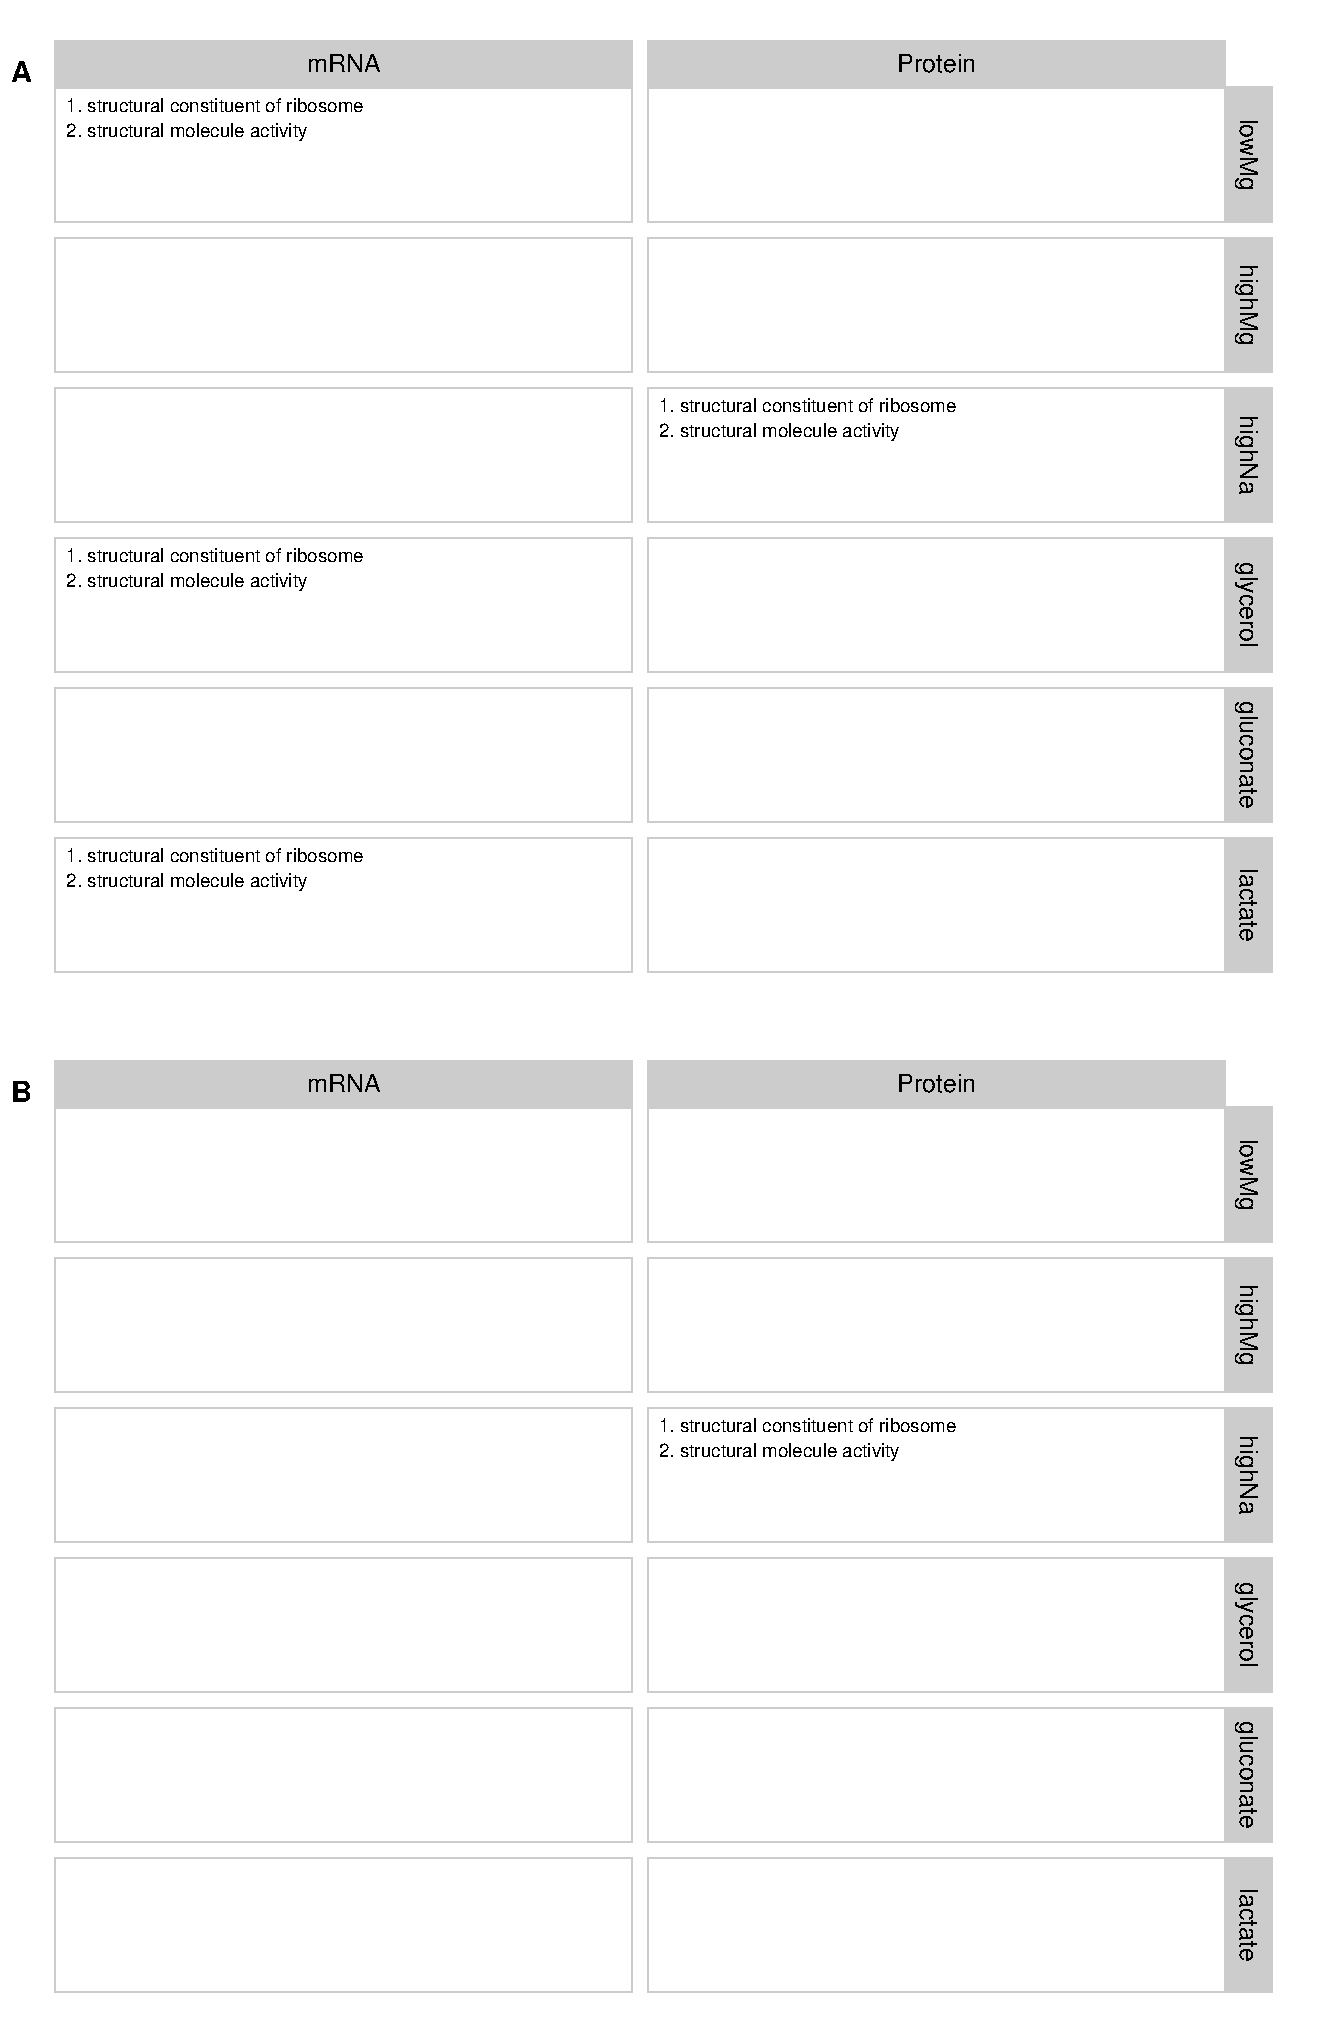
\includegraphics[width=0.85\textwidth]{../supplementary_figures/figS1_ResultSumamryFigures_mf.pdf}
	\caption[Summary GO annotations]
	{\textbf{Significantly differentially expressed Molecular Functions generated by GO annotations.} For each condition, we show the top-5 differentially expressed MF as determined by either mRNA or protein abundances. (A) exponential phase. (B) stationary phase.}
\end{figure}

\clearpage

\begin{figure}[!htb]
	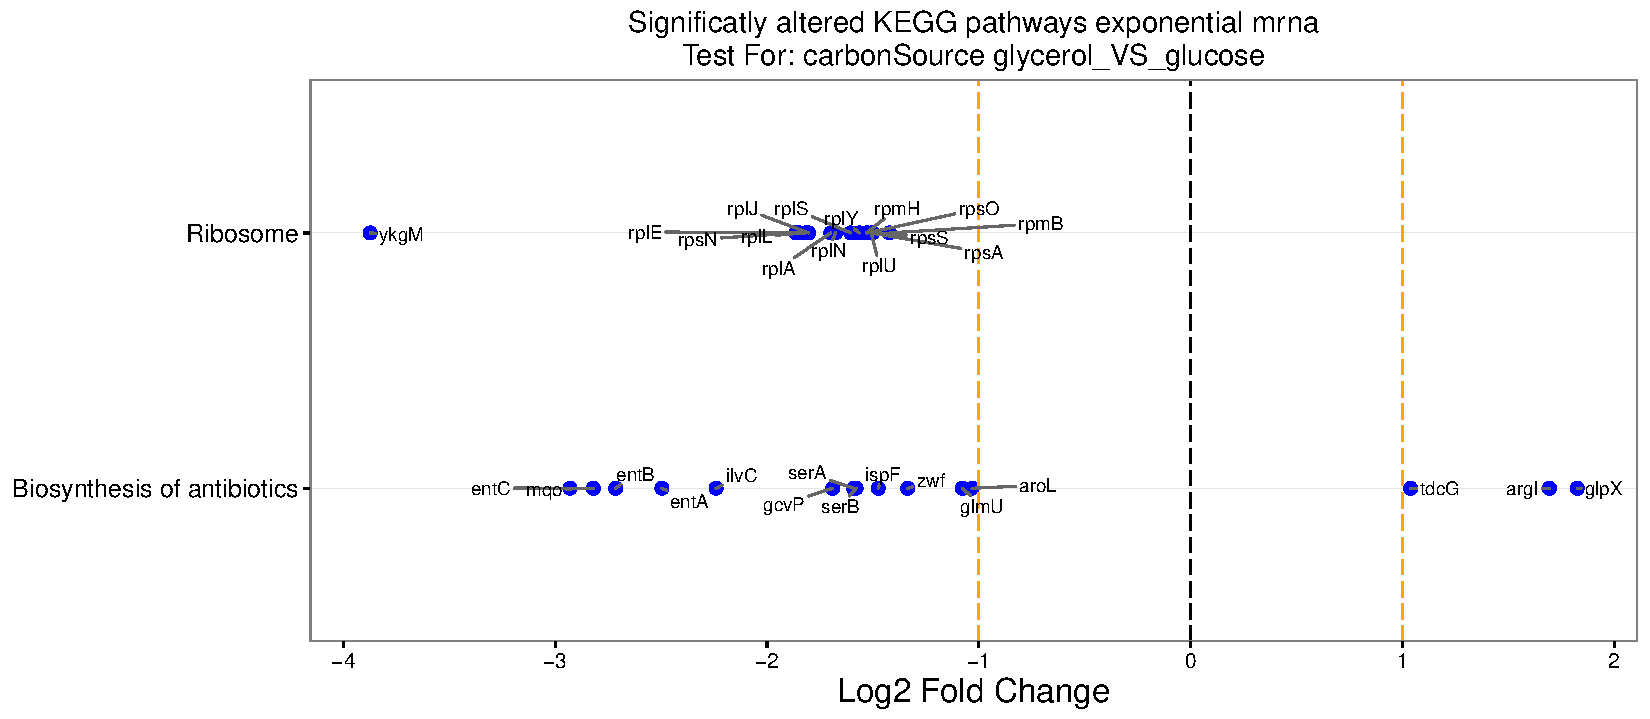
\includegraphics[width=1.0\textwidth]{../../d_figures/kegg_01.pdf}
	\caption[Significantly altered KEGG pathways for mRNA samples in exponential phase tested for glycerol against glucose]
	{\textbf{Significantly differentially expressed KEGG pathways and associated genes with glycerol as carbon source in exponential phase, as determined by mRNA abundances.} The top differentially expressed KEGG pathways are shown along the y axis, and the relative fold change of the corresponding genes is shown along the x axis. In figure we show up to 10 most significantly changed pathways and for each pathway we show up to 15 of the most significantly changing genes.}
\end{figure}

\clearpage
\begin{figure}
	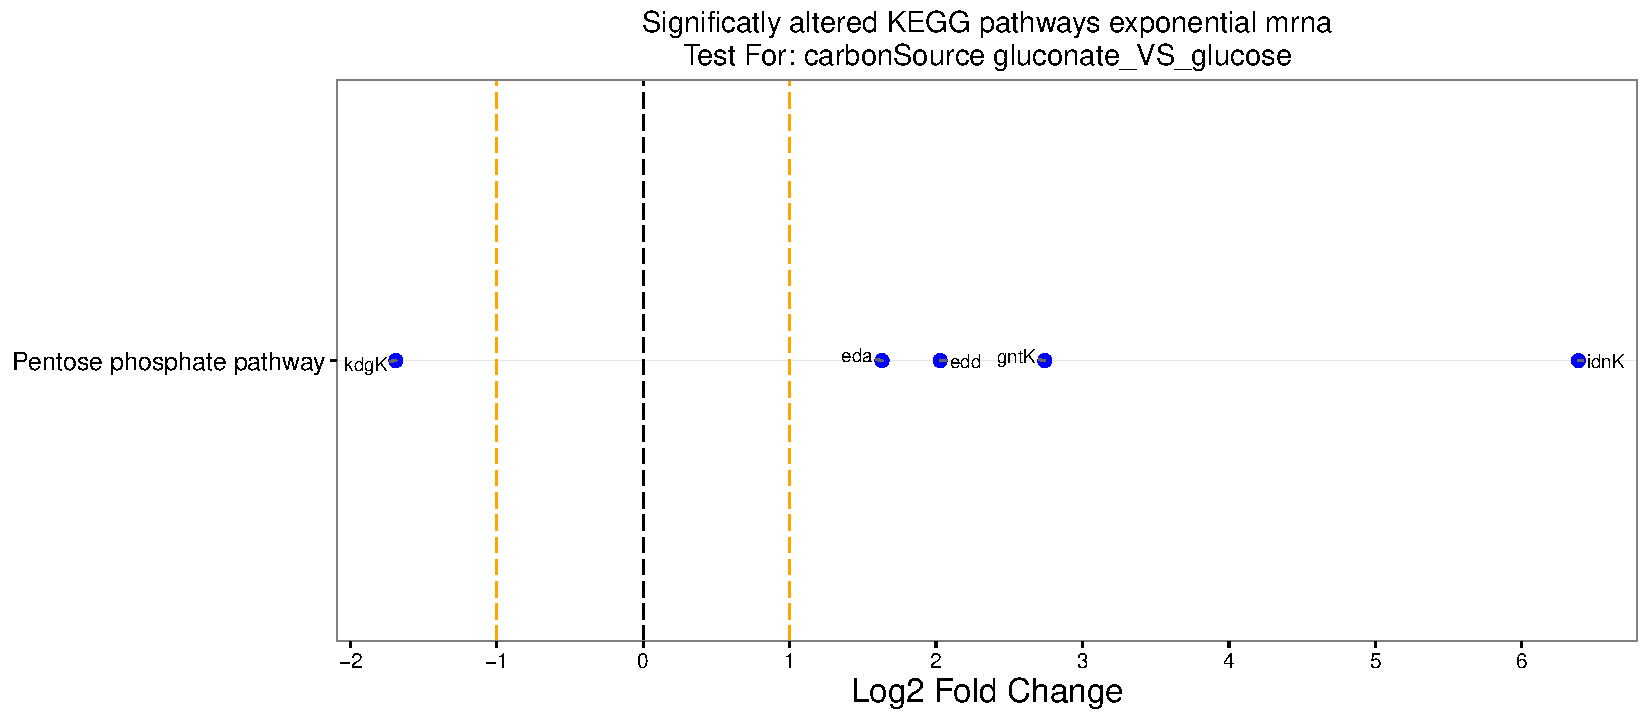
\includegraphics[width=1.0\textwidth]{../../d_figures/kegg_02.pdf}
	\caption[Significantly altered KEGG pathways for mRNA samples in exponential phase tested for  against glucose]
	{\textbf{Significantly differentially expressed KEGG pathways and associated genes with gluconate as carbon source in exponential phase, as determined by mRNA abundances.} The top differentially expressed KEGG pathways are shown along the y axis, and the relative fold change of the corresponding genes is shown along the x axis. In figure we show up to 10 most significantly changed pathways and for each pathway we show up to 15 of the most significantly changing genes.}
\end{figure}

\clearpage
\begin{figure}
	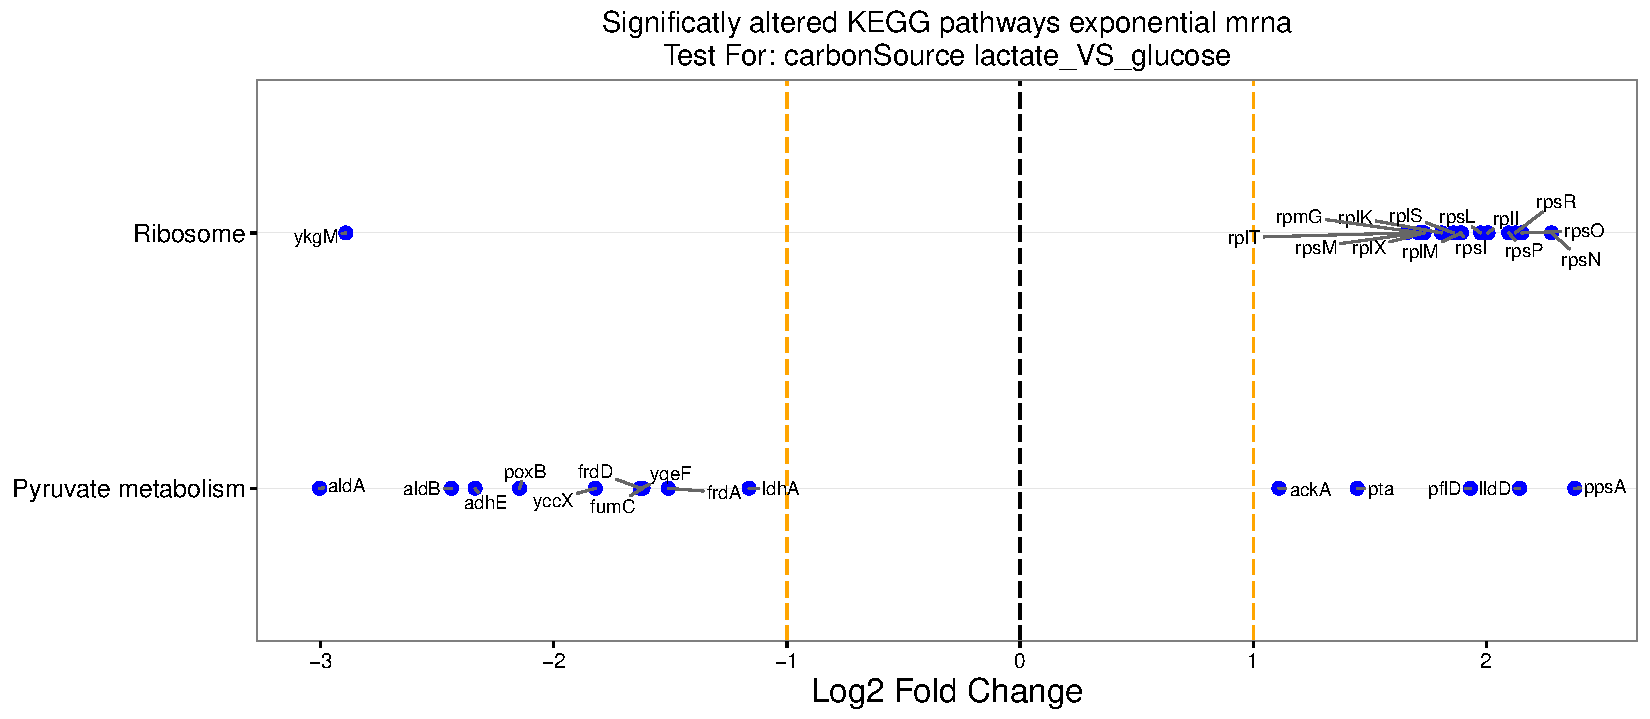
\includegraphics[width=1.0\textwidth]{../../d_figures/kegg_03.pdf}
	\caption[Significantly altered KEGG pathways for mRNA samples in exponential phase tested for lactate against glucose]
	{\textbf{Significantly differentially expressed KEGG pathways and associated genes with lactate as carbon source in exponential phase, as determined by mRNA abundances.} The top differentially expressed KEGG pathways are shown along the y axis, and the relative fold change of the corresponding genes is shown along the x axis. In figure we show up to 10 most significantly changed pathways and for each pathway we show up to 15 of the most significantly changing genes.}
\end{figure}

\clearpage
\begin{figure}
	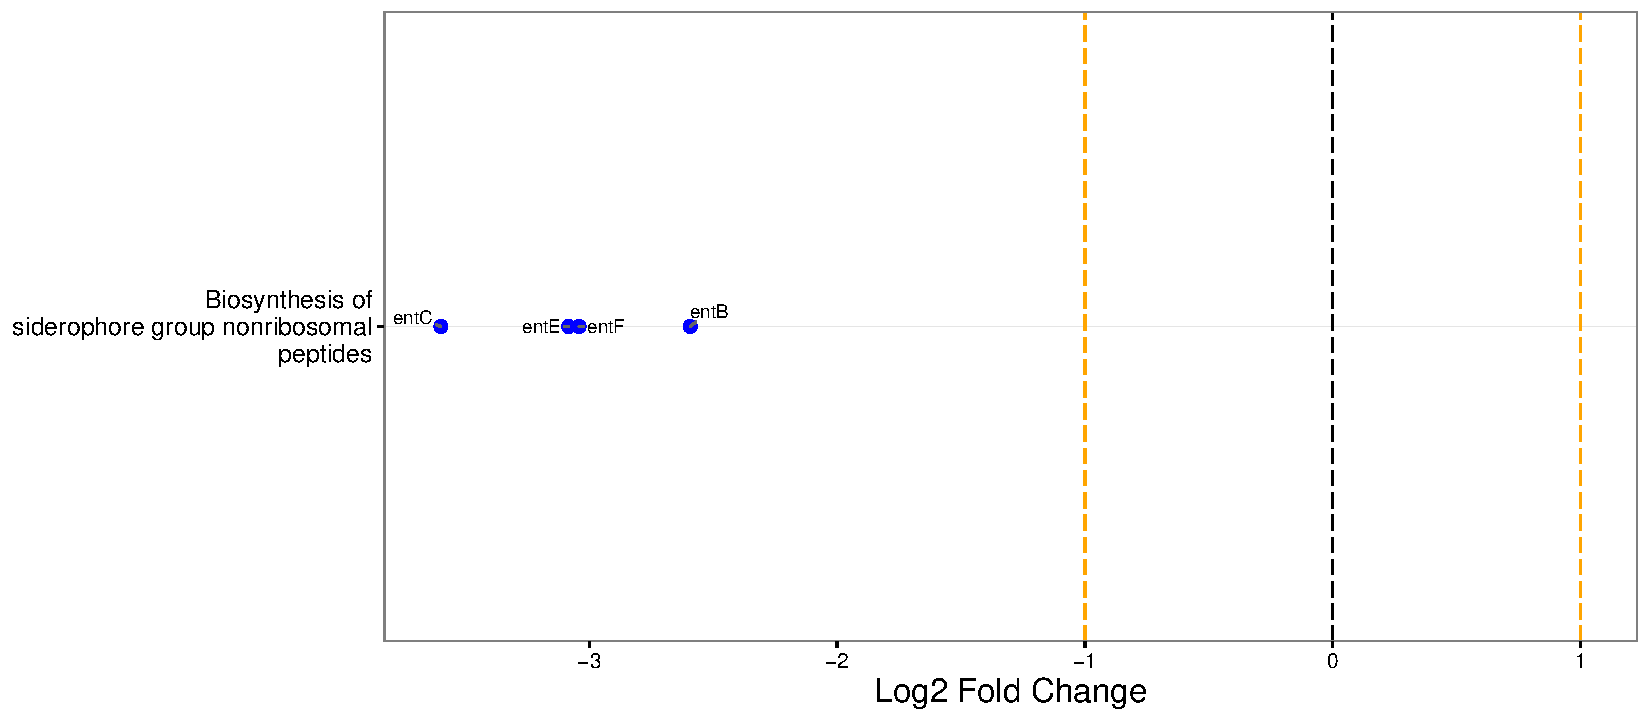
\includegraphics[width=1.0\textwidth]{../../d_figures/kegg_04.pdf}
	\caption[Significantly altered KEGG pathways for protein samples in exponential phase tested for gluconate against glucose]
	{\textbf{Significantly differentially expressed KEGG pathways and associated genes with gluconate as carbon source in exponential phase, as determined by protein abundances.} The top differentially expressed KEGG pathways are shown along the y axis, and the relative fold change of the corresponding genes is shown along the x axis. In figure we show up to 10 most significantly changed pathways and for each pathway we show up to 15 of the most significantly changing genes.}
\end{figure}

\clearpage
\begin{figure}
	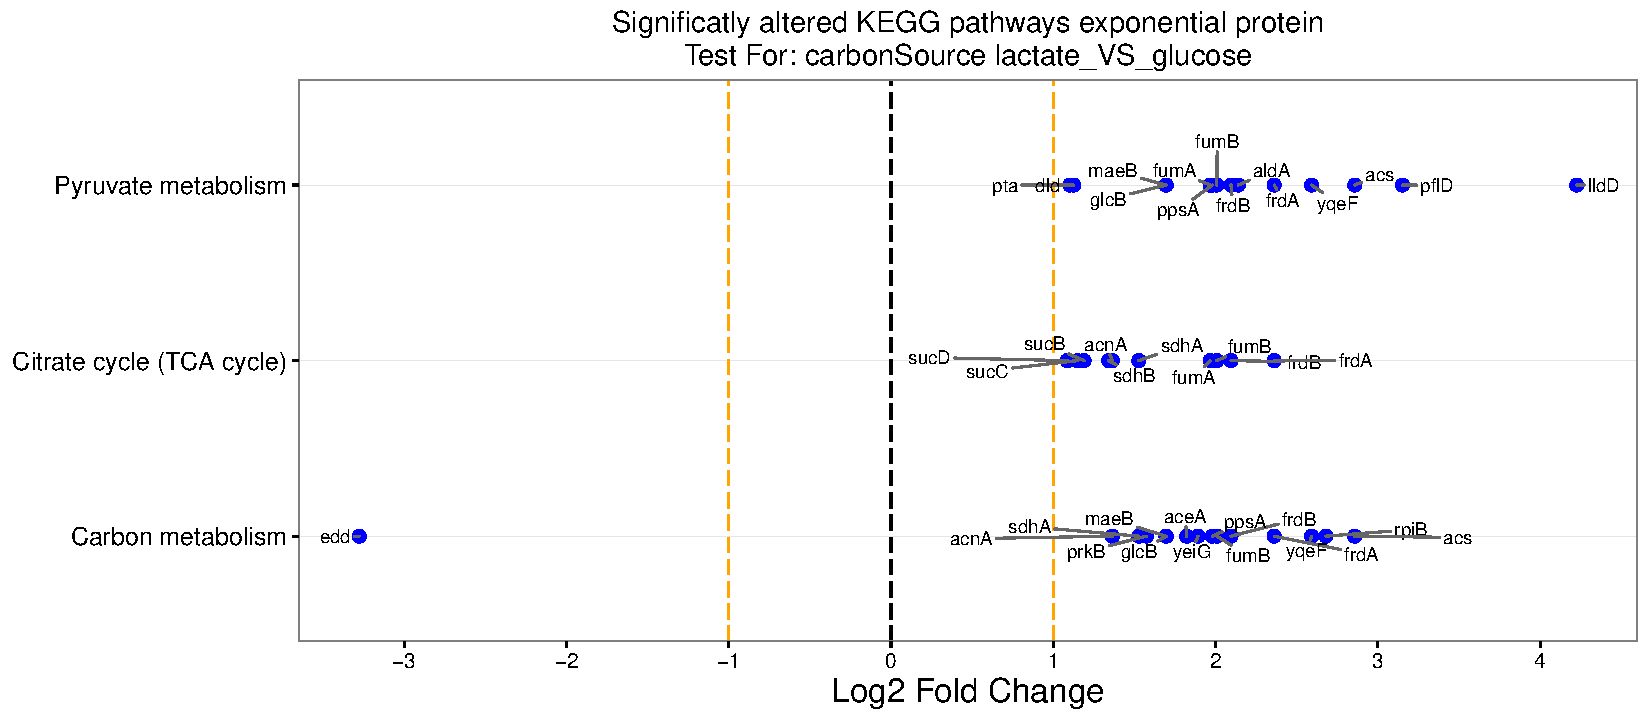
\includegraphics[width=1.0\textwidth]{../../d_figures/kegg_05.pdf}
	\caption[Significantly altered KEGG pathways for protein samples in exponential phase tested for lactate against glucose]
	{\textbf{Significantly differentially expressed KEGG pathways and associated genes with lactate as carbon source in exponential phase, as determined by protein abundances.} The top differentially expressed KEGG pathways are shown along the y axis, and the relative fold change of the corresponding genes is shown along the x axis. In figure we show up to 10 most significantly changed pathways and for each pathway we show up to 15 of the most significantly changing genes.}
\end{figure}

\clearpage
\begin{figure}
	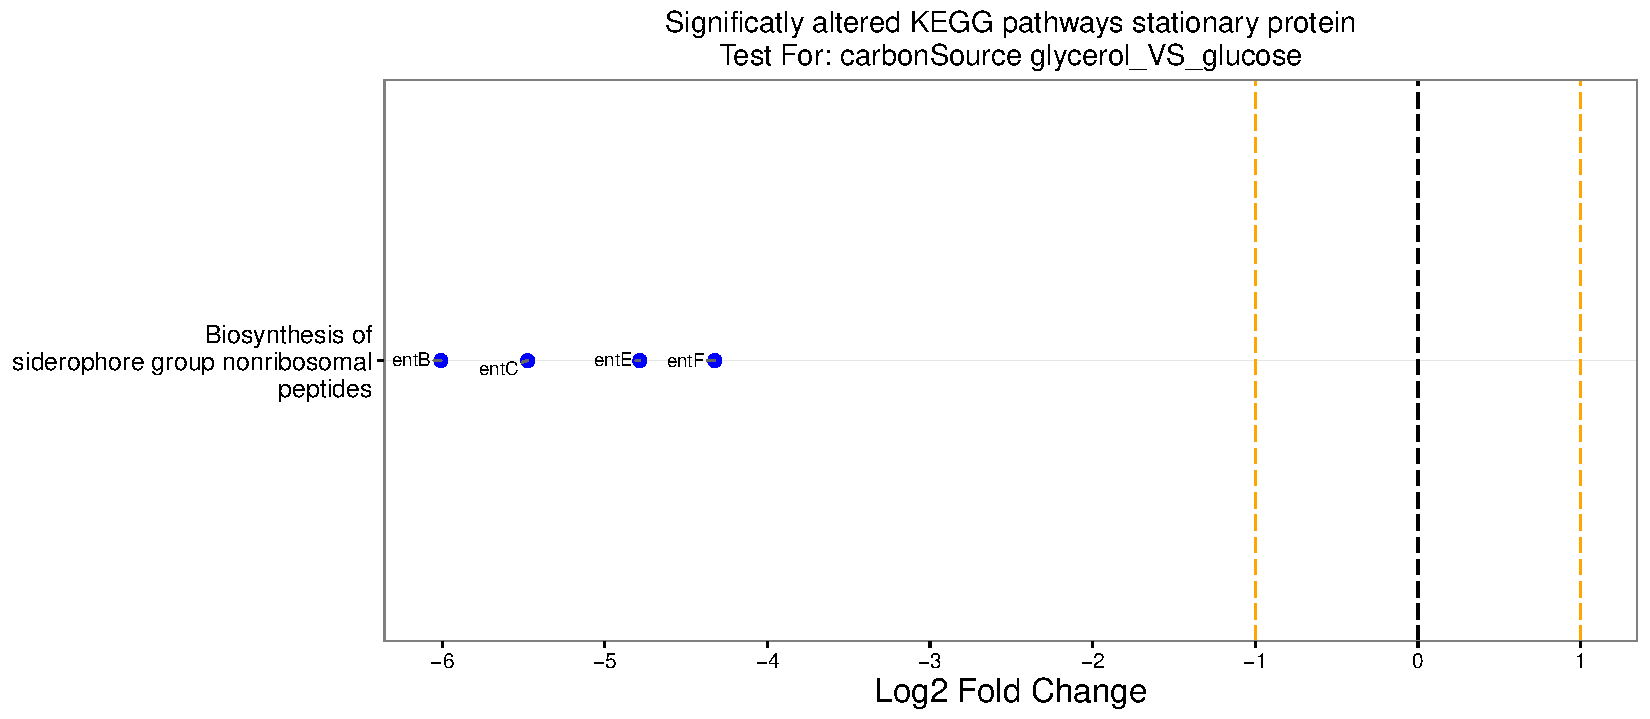
\includegraphics[width=1.0\textwidth]{../../d_figures/kegg_06.pdf}
	\caption[Significantly altered KEGG pathways for protein samples in stationary phase tested for glycerol against glucose]
	{\textbf{Significantly differentially expressed KEGG pathways and associated genes with glycerol as carbon source in stationary phase, as determined by protein abundances.} The top differentially expressed KEGG pathways are shown along the y axis, and the relative fold change of the corresponding genes is shown along the x axis. In figure we show up to 10 most significantly changed pathways and for each pathway, we show up to 15 of the most significantly changing genes.}
\end{figure}

\clearpage
\begin{figure}
	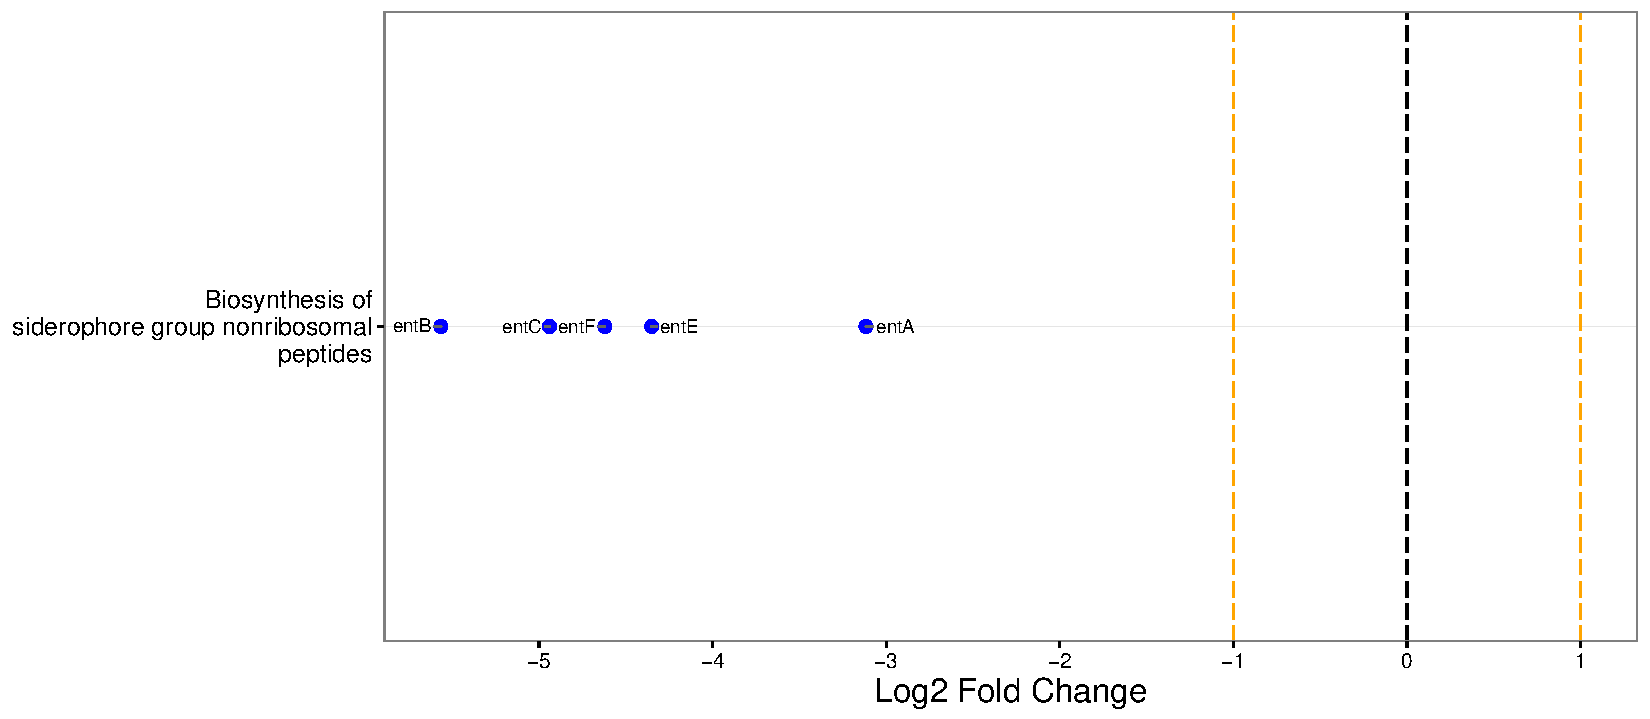
\includegraphics[width=1.0\textwidth]{../../d_figures/kegg_07.pdf}
	\caption[Significantly altered KEGG pathways for protein samples in stationary phase tested for gluconate against glucose]
	{\textbf{Significantly differentially expressed KEGG pathways and associated genes with gluconate as carbon source in stationary phase, as determined by protein abundances.} The top differentially expressed KEGG pathways are shown along the y axis, and the relative fold change of the corresponding genes is shown along the x axis. We show up to 10 most significantly changed pathways and for each pathway, we show up to 15 of the most significantly changing genes.}
\end{figure}

\clearpage
\begin{figure}
	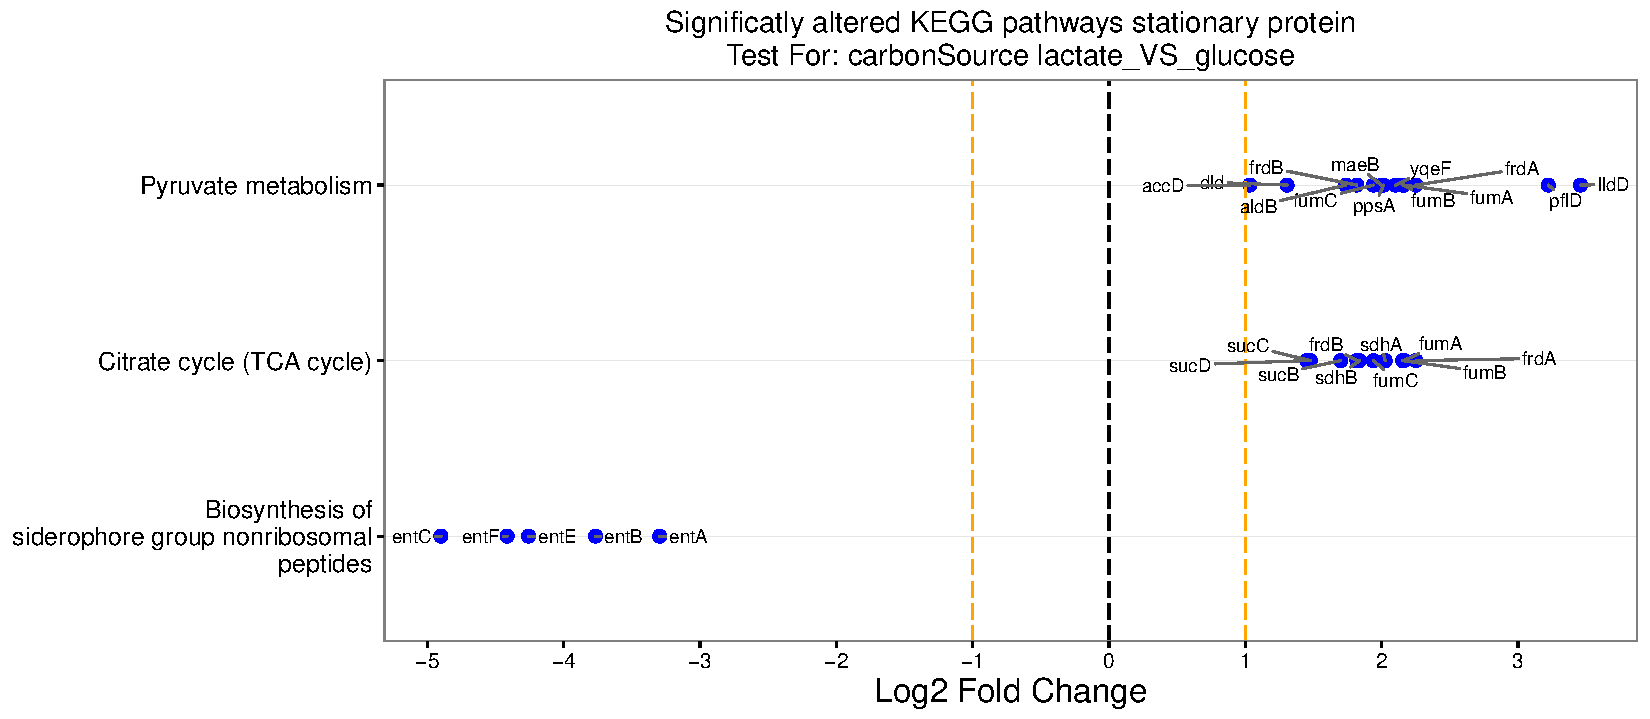
\includegraphics[width=1.0\textwidth]{../../d_figures/kegg_08.pdf}
	\caption[Significantly altered KEGG pathways for protein samples in stationary phase tested for lactate against glucose]
	{\textbf{Significantly differentially expressed KEGG pathways and associated genes with lactate as carbon source in stationary phase, as determined by protein abundances.} The top differentially expressed KEGG pathways are shown along the y axis, and the relative fold change of the corresponding genes is shown along the x axis. We show up to 10 most significantly changed pathways and for each pathway, we show up to 15 of the most significantly changing genes.}
\end{figure}

\clearpage
\begin{figure}
	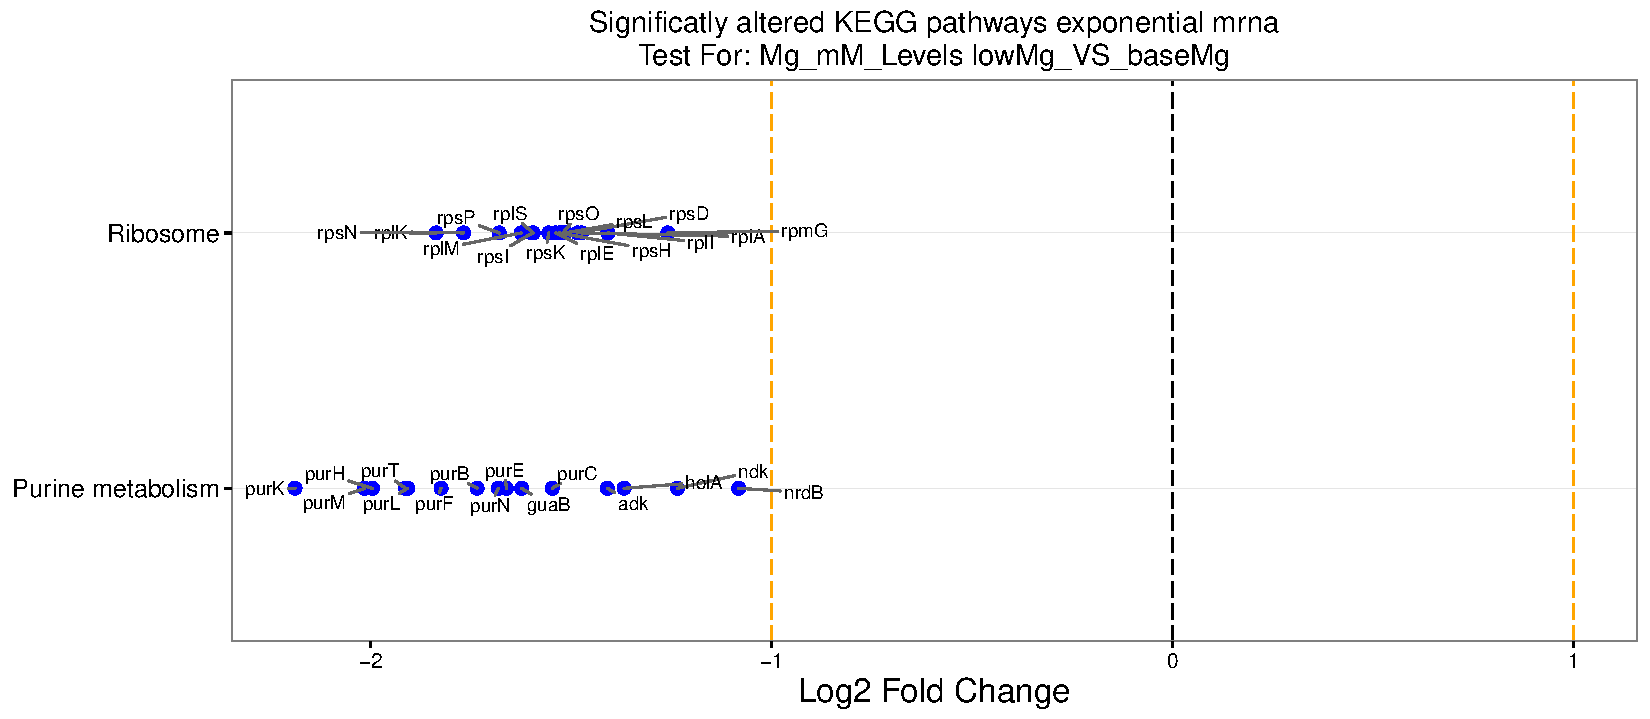
\includegraphics[width=1.0\textwidth]{../../d_figures/kegg_09.pdf}
	\caption[Significantly altered KEGG pathways for mRNA samples in exponential phase tested for low Mg\textsuperscript{+2} levels against base Mg\textsuperscript{+2}]
	{\textbf{Significantly differentially expressed KEGG pathways and associated genes with low Mg\textsuperscript{+2} levels in exponential phase, as determined by mRNA abundances.} The top differentially expressed KEGG pathways are shown along the y axis, and the relative fold change of the corresponding genes is shown along the x axis. We show up to 10 most significantly changed pathways and for each pathway, we show up to 15 of the most significantly changing genes.}
\end{figure}

\clearpage
\begin{figure}
	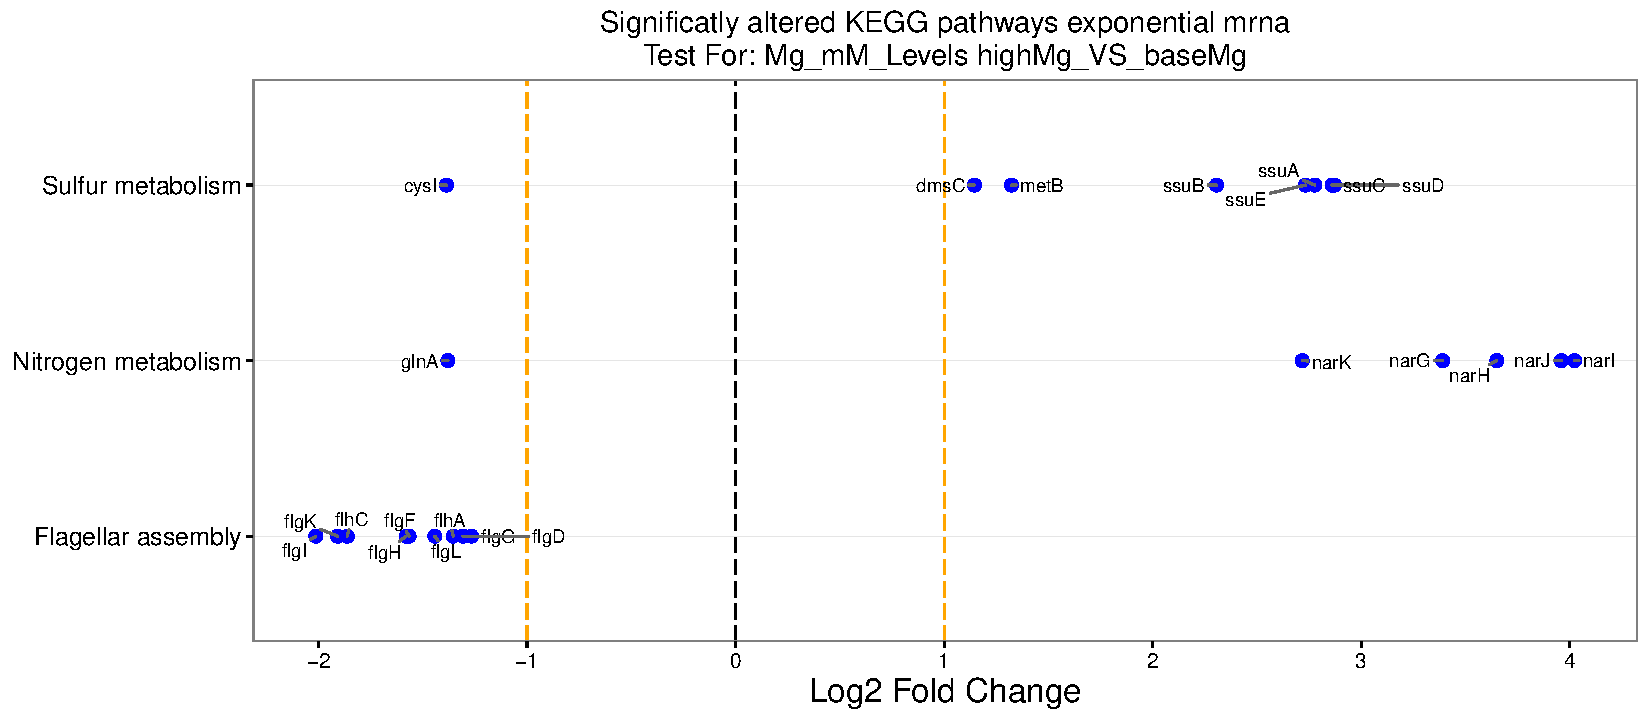
\includegraphics[width=1.0\textwidth]{../../d_figures/kegg_10.pdf}
	\caption[Significantly altered KEGG pathways for mRNA samples in exponential phase tested for high Mg\textsuperscript{+2} against base Mg\textsuperscript{+2}]
	{\textbf{Significantly differentially expressed KEGG pathways and associated genes with high Mg\textsuperscript{+2} levels in exponential phase, as determined by mRNA abundances.} The top differentially expressed KEGG pathways are shown along the y axis, and the relative fold change of the corresponding genes is shown along the x axis. We show up to 10 most significantly changed pathways and for each pathway, we show up to 15 of the most significantly changing genes.}
\end{figure}

\clearpage
\begin{figure}
	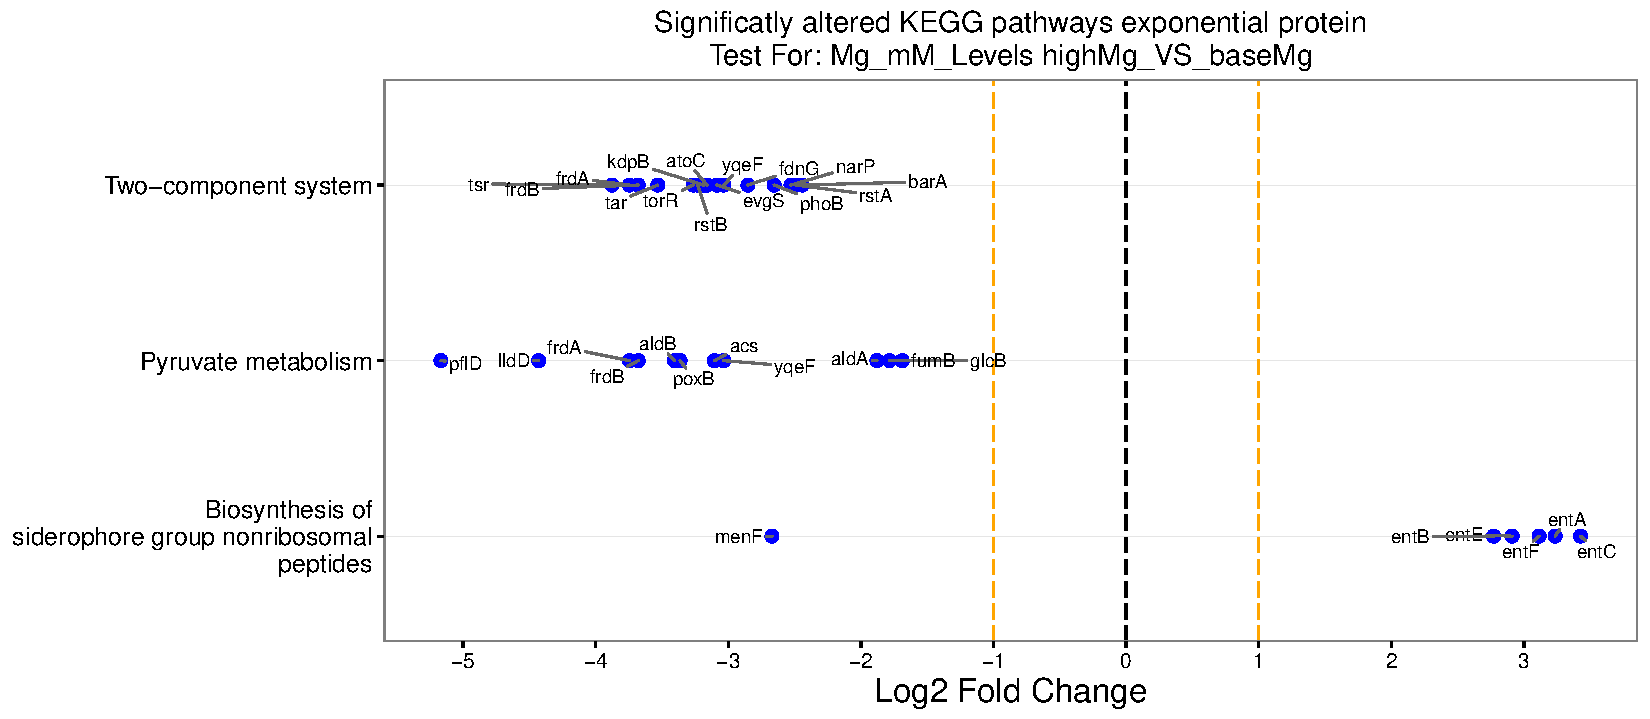
\includegraphics[width=1.0\textwidth]{../../d_figures/kegg_11.pdf}
	\caption[Significantly altered KEGG pathways for protein samples in exponential phase tested for high Mg\textsuperscript{+2} against base Mg\textsuperscript{+2}]
	{\textbf{Significantly differentially expressed KEGG pathways and associated genes with high Mg\textsuperscript{+2} levels in exponential phase, as determined by protein abundances.} The top differentially expressed KEGG pathways are shown along the y axis, and the relative fold change of the corresponding genes is shown along the x axis. We show up to 10 most significantly changed pathways and for each pathway, we show up to 15 of the most significantly changing genes.}
\end{figure}

\clearpage
\begin{figure}
	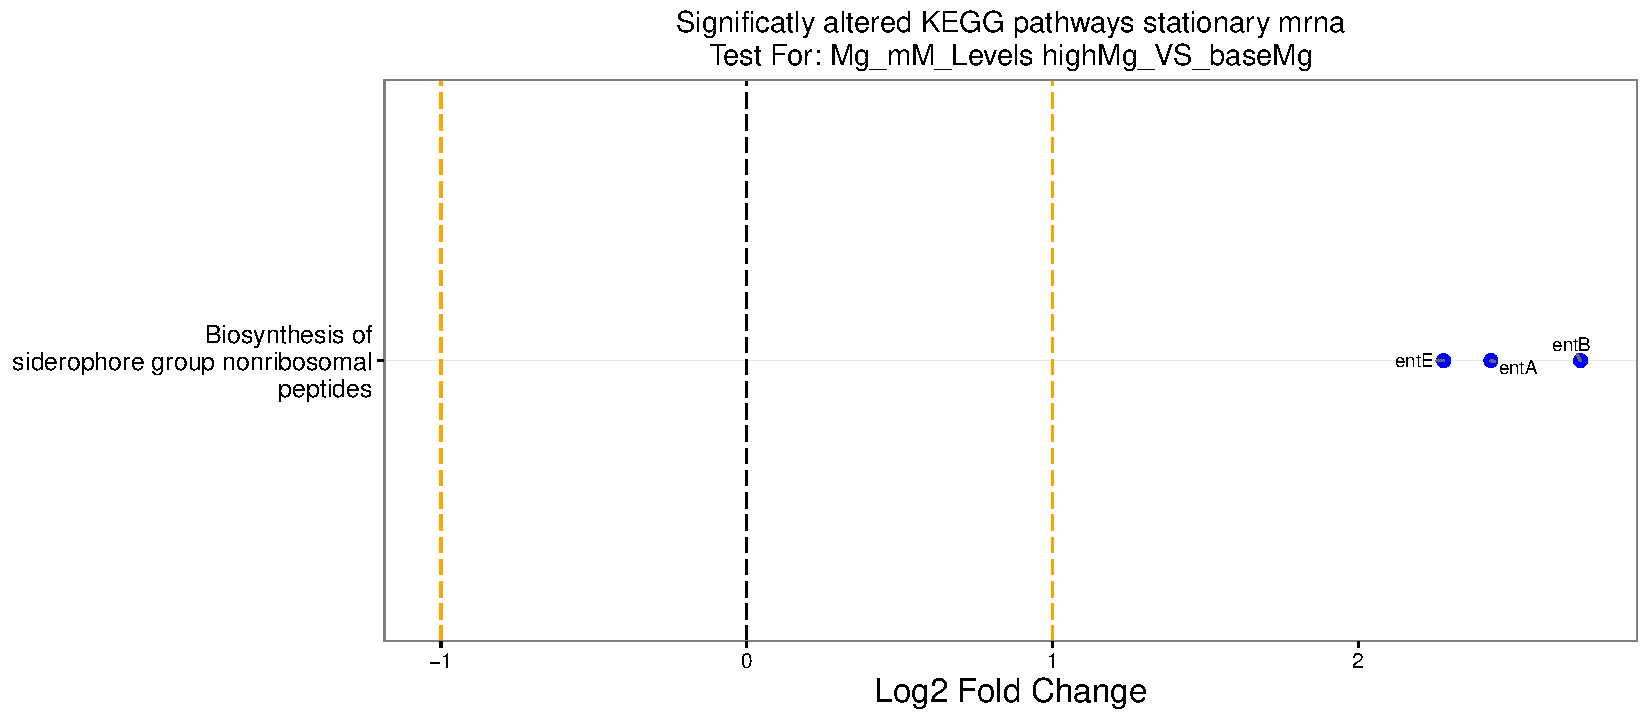
\includegraphics[width=1.0\textwidth]{../../d_figures/kegg_12.pdf}
	\caption[Significantly altered KEGG pathways for mRNA samples in stationary phase tested for high Mg\textsuperscript{+2} against base Mg\textsuperscript{+2}]
	{\textbf{Significantly differentially expressed KEGG pathways and associated genes with high Mg\textsuperscript{+2} levels in stationary phase, as determined by mRNA abundances.} The top differentially expressed KEGG pathways are shown along the y axis, and the relative fold change of the corresponding genes is shown along the x axis. We show up to 10 most significantly changed pathways and for each pathway, we show up to 15 of the most significantly changing genes.}
\end{figure}

\clearpage
\begin{figure}
	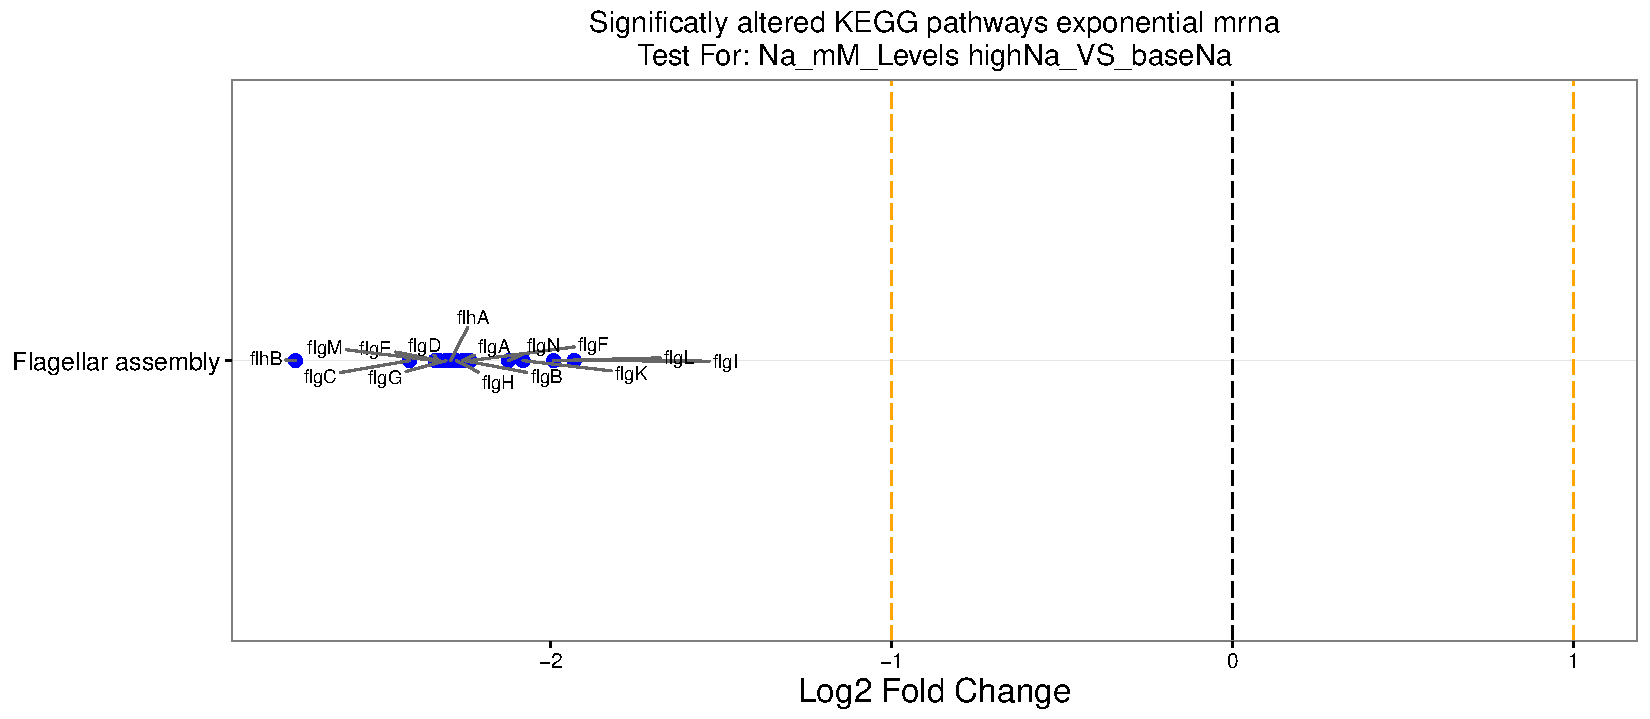
\includegraphics[width=1.0\textwidth]{../../d_figures/kegg_13.pdf}
	\caption[Significantly altered KEGG pathways for mRNA samples in exponential phase tested for high Na\textsuperscript{+1} against base Na\textsuperscript{+1}]
	{\textbf{Significantly differentially expressed KEGG pathways and associated genes with high Na\textsuperscript{+1} levels in exponential phase, as determined by mRNA abundances.} The top differentially expressed KEGG pathways are shown along the y axis, and the relative fold change of the corresponding genes is shown along the x axis. We show up to 10 most significantly changed pathways and for each pathway, we show up to 15 of the most significantly changing genes.}
\end{figure}

\clearpage
\begin{figure}
	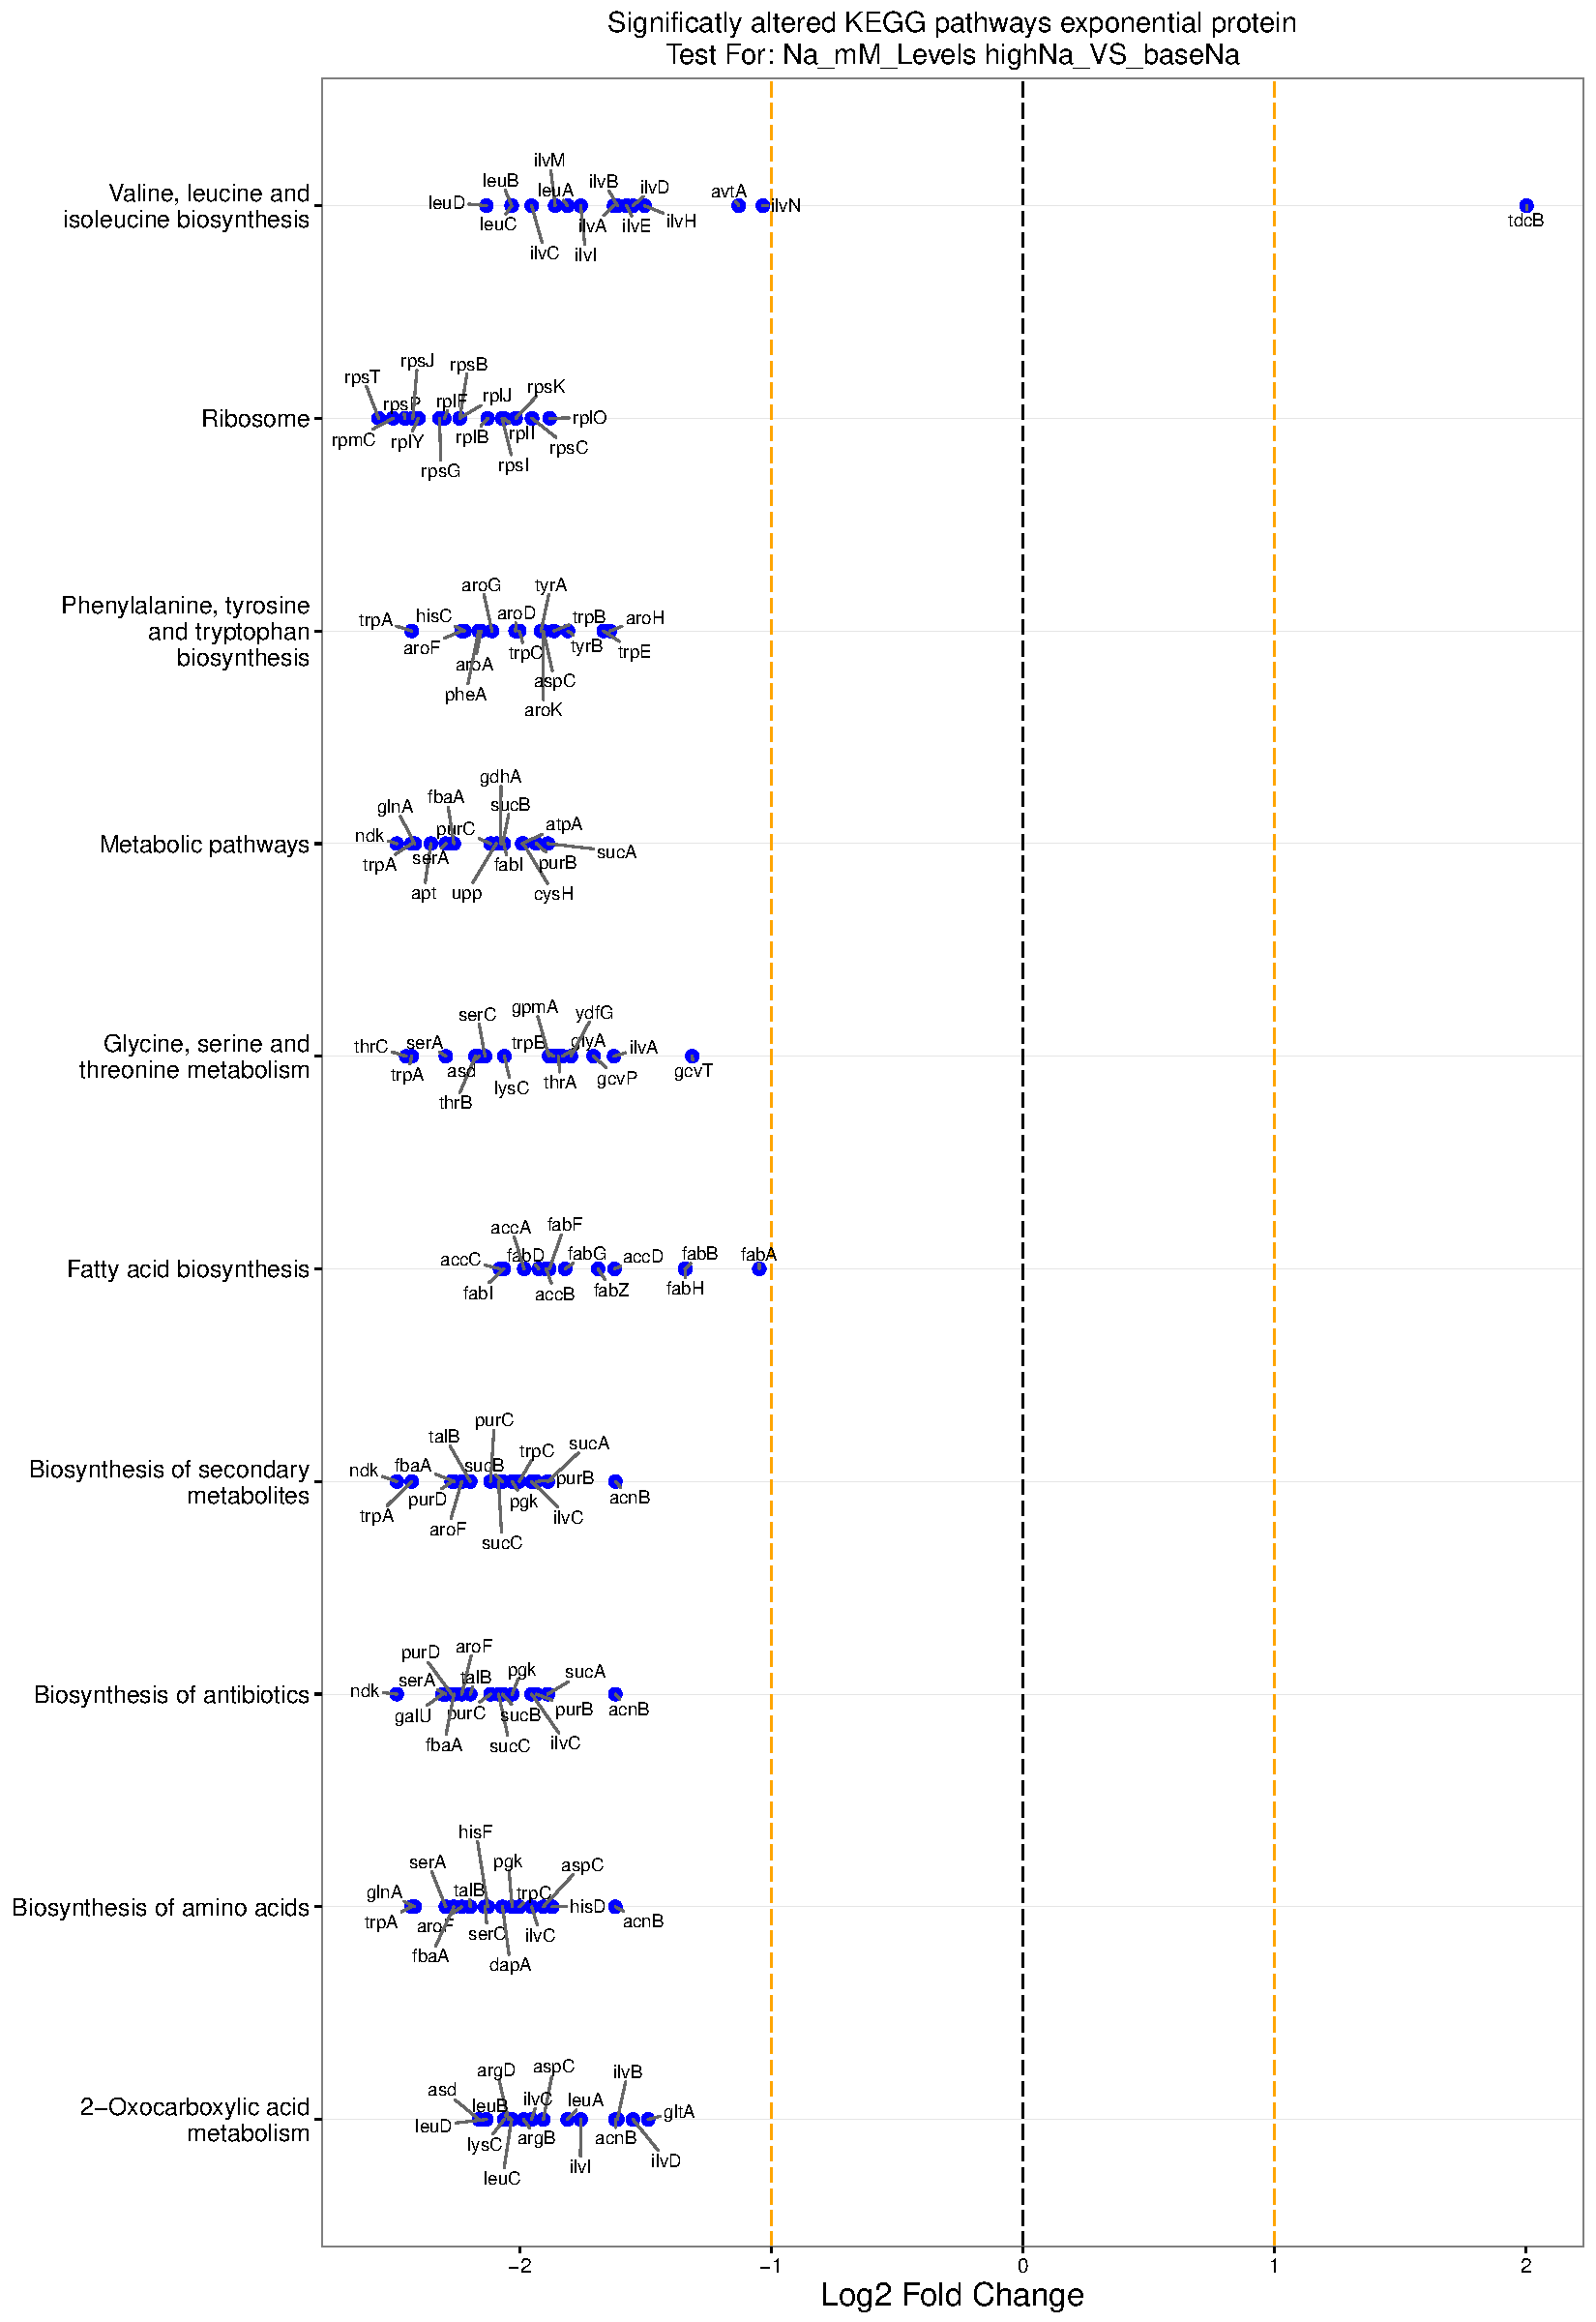
\includegraphics[width=1.0\textwidth]{../../d_figures/kegg_14.pdf}
	\caption[Significantly altered KEGG pathways for protein samples in exponential phase tested for high Na\textsuperscript{+1} against base Na\textsuperscript{+1}]
	{\textbf{Significantly differentially expressed KEGG pathways and associated genes with high Na\textsuperscript{+1} levels in exponential phase, as determined by protein abundances.} The top differentially expressed KEGG pathways are shown along the y axis, and the relative fold change of the corresponding genes is shown along the x axis. We show up to 10 most significantly changed pathways and for each pathway, we show up to 15 of the most significantly changing genes.}
\end{figure}

\clearpage
\begin{figure}
	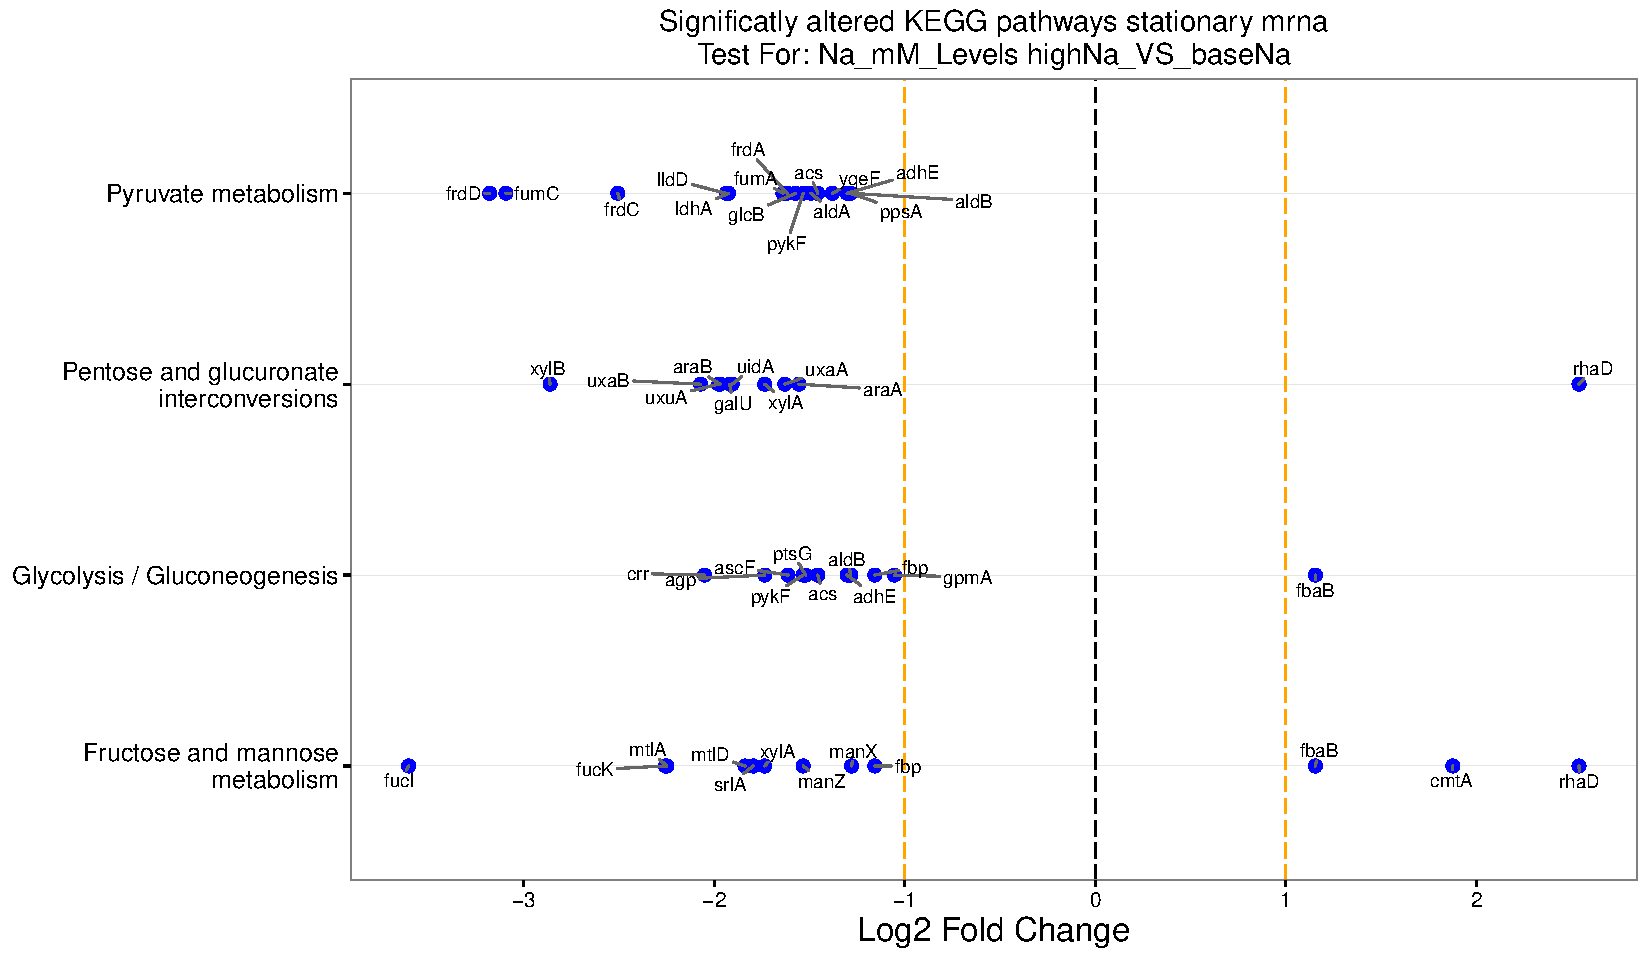
\includegraphics[width=1.0\textwidth]{../../d_figures/kegg_15.pdf}
	\caption[Significantly altered KEGG pathways for mRNA samples in stationary phase tested for high Na\textsuperscript{+1} against base Na\textsuperscript{+1}]
	{\textbf{Significantly differentially expressed KEGG pathways and associated genes with high Na\textsuperscript{+1} levels in stationary phase, as determined by mRNA abundances.} The top differentially expressed KEGG pathways are shown along the y axis, and the relative fold change of the corresponding genes is shown along the x axis. We show up to 10 most significantly changed pathways and for each pathway, we show up to 15 of the most significantly changing genes.}
\end{figure}

\clearpage
\begin{figure}
	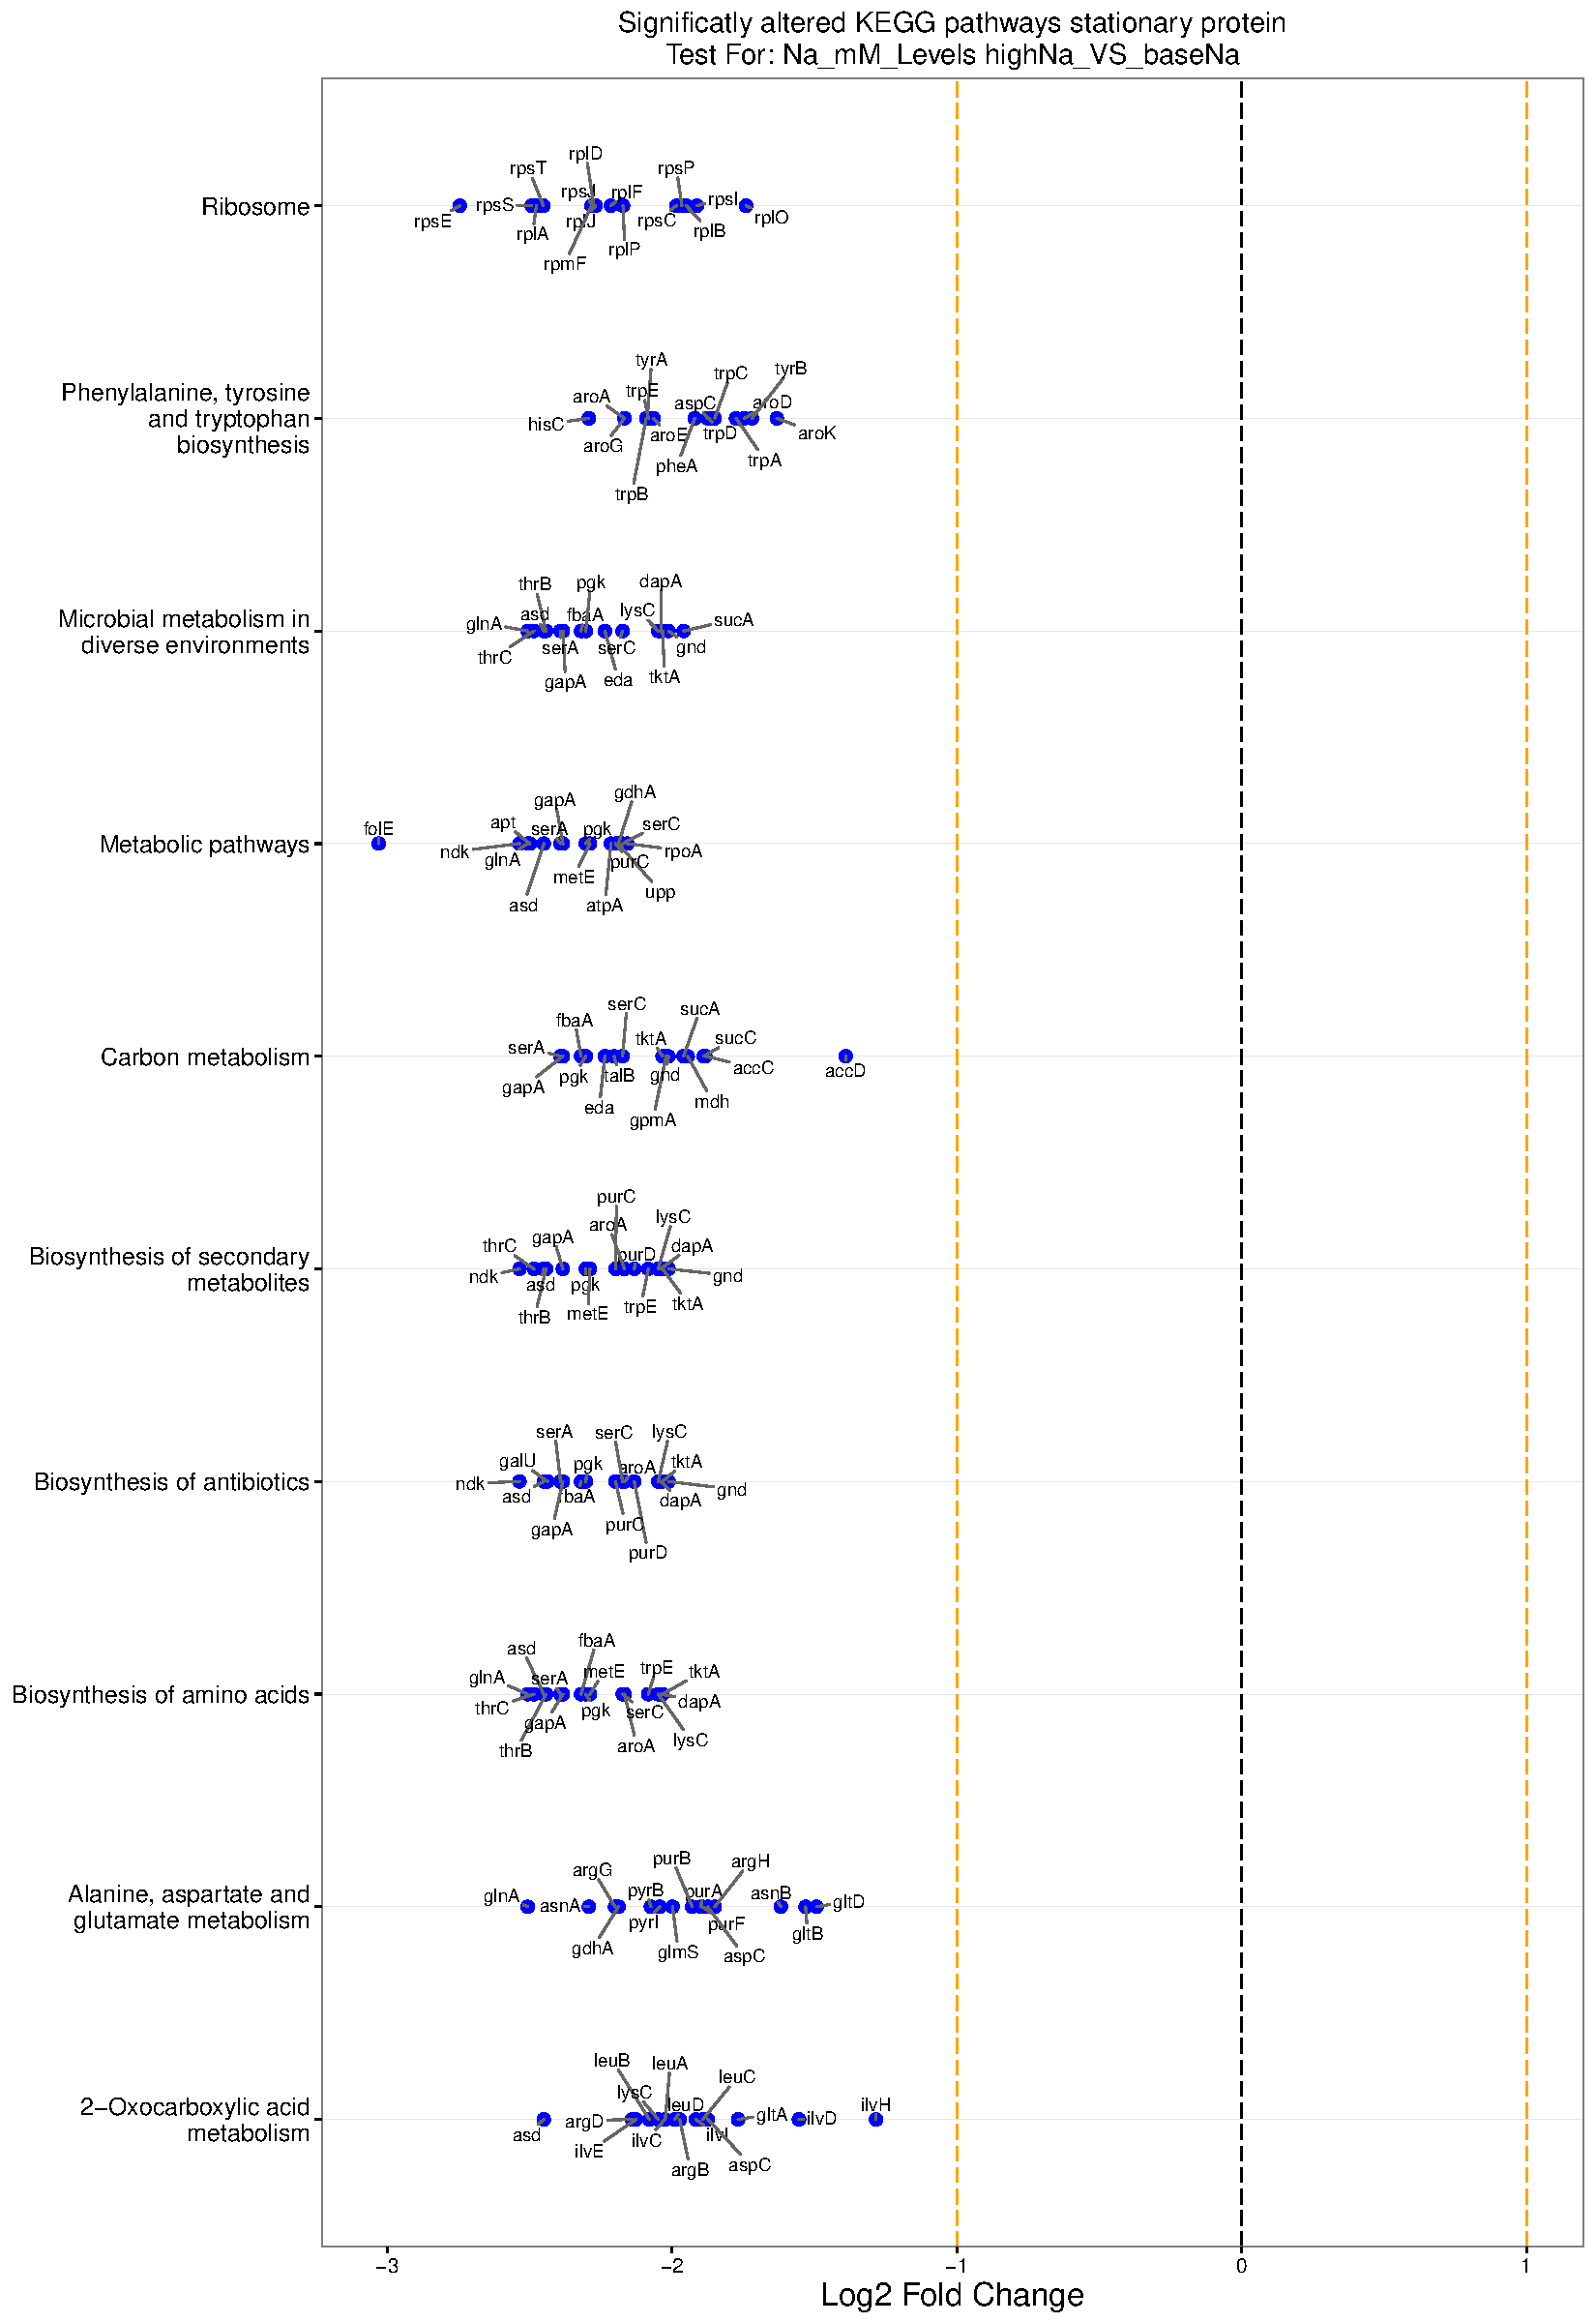
\includegraphics[width=1.0\textwidth]{../../d_figures/kegg_16.pdf}
	\caption[Significantly altered KEGG pathways for protein samples in stationary phase tested for high Na\textsuperscript{+1} against base Na\textsuperscript{+1}]
	{\textbf{Significantly differentially expressed KEGG pathways and associated genes with high Na\textsuperscript{+1} levels in stationary phase, as determined by protein abundances.} The top differentially expressed KEGG pathways are shown along the y axis, and the relative fold change of the corresponding genes is shown along the x axis. We show up to 10 most significantly changed pathways and for each pathway, we show up to 15 of the most significantly changing genes.}
\end{figure}
\clearpage


\begin{figure}[!htb]
	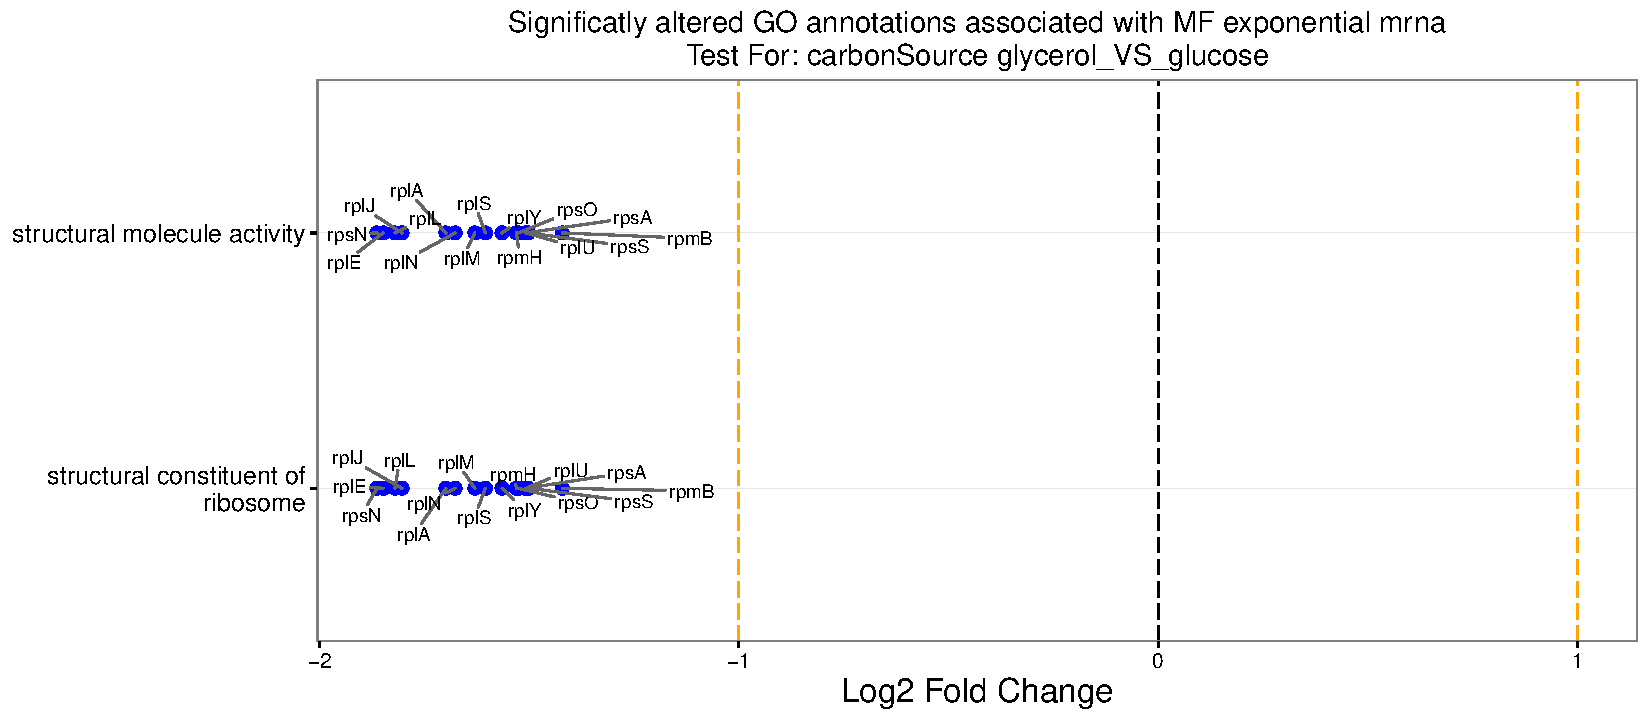
\includegraphics[width=1.0\textwidth]{../../d_figures/mf_n_01.pdf}
	\caption[Significantly altered GO annotations associated with molecular functions for mRNA samples in exponential phase tested for glycerol against glucose]
	{\textbf{Significantly differentially expressed GO annotations related with molecular functions and associated genes with glycerol as carbon source in exponential phase, as determined by mRNA abundances.} The top differentially expressed KEGG pathways are shown along the y axis, and the relative fold change of the corresponding genes is shown along the x axis. We show up to 10 most significantly changed pathways and for each pathway, we show up to 15 of the most significantly changing genes.}
\end{figure}

\clearpage
\begin{figure}
	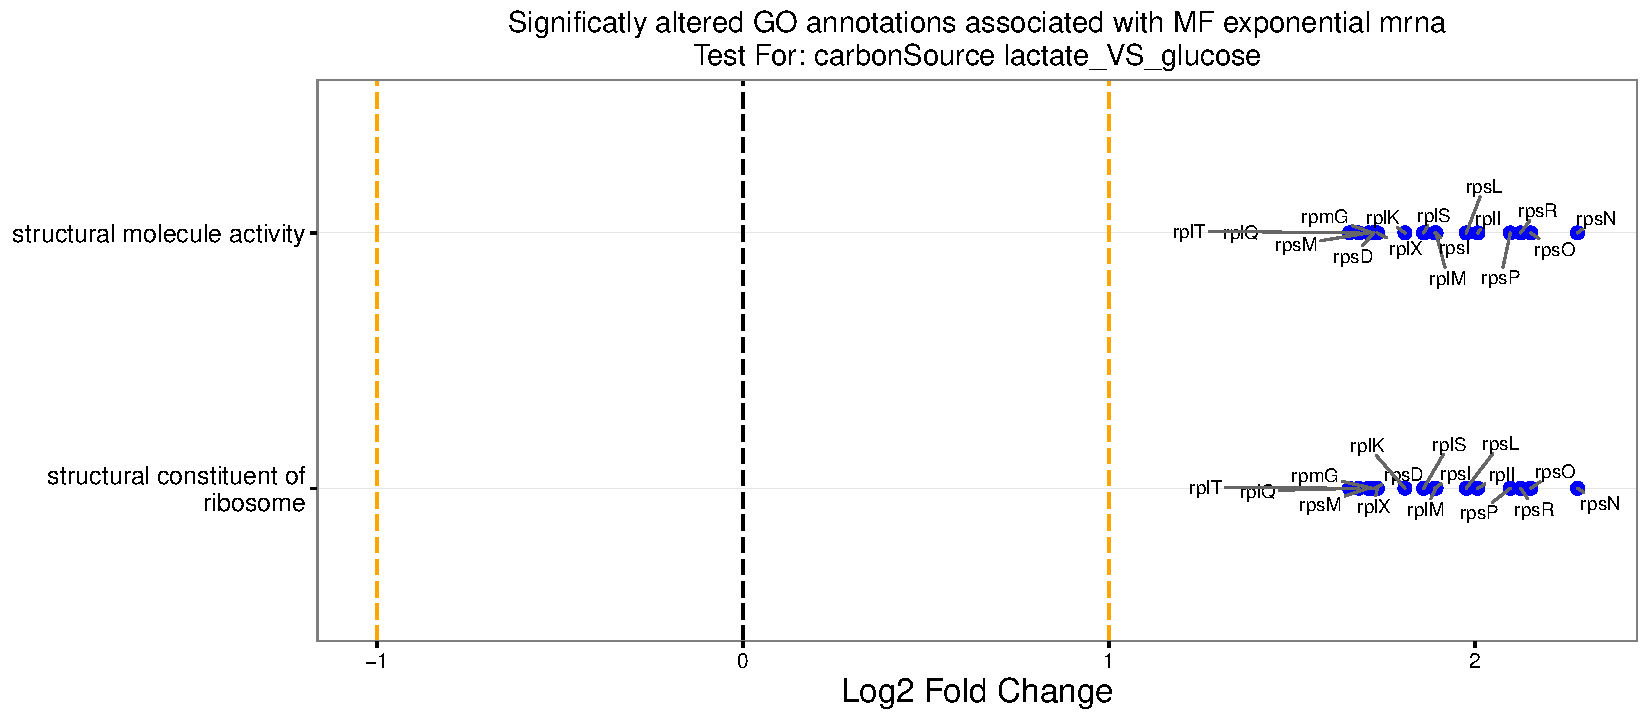
\includegraphics[width=1.0\textwidth]{../../d_figures/mf_n_02.pdf}
	\caption[Significantly altered GO annotations associated with molecular functions for mRNA samples in exponential phase tested for lactate against glucose]
	{\textbf{Significantly differentially expressed GO annotations related with molecular functions and associated genes with lactate as carbon source in exponential phase, as determined by mRNA abundances.} The top differentially expressed KEGG pathways are shown along the y axis, and the relative fold change of the corresponding genes is shown along the x axis. We show up to 10 most significantly changed pathways and for each pathway, we show up to 15 of the most significantly changing genes.}
\end{figure}

\clearpage
\begin{figure}
	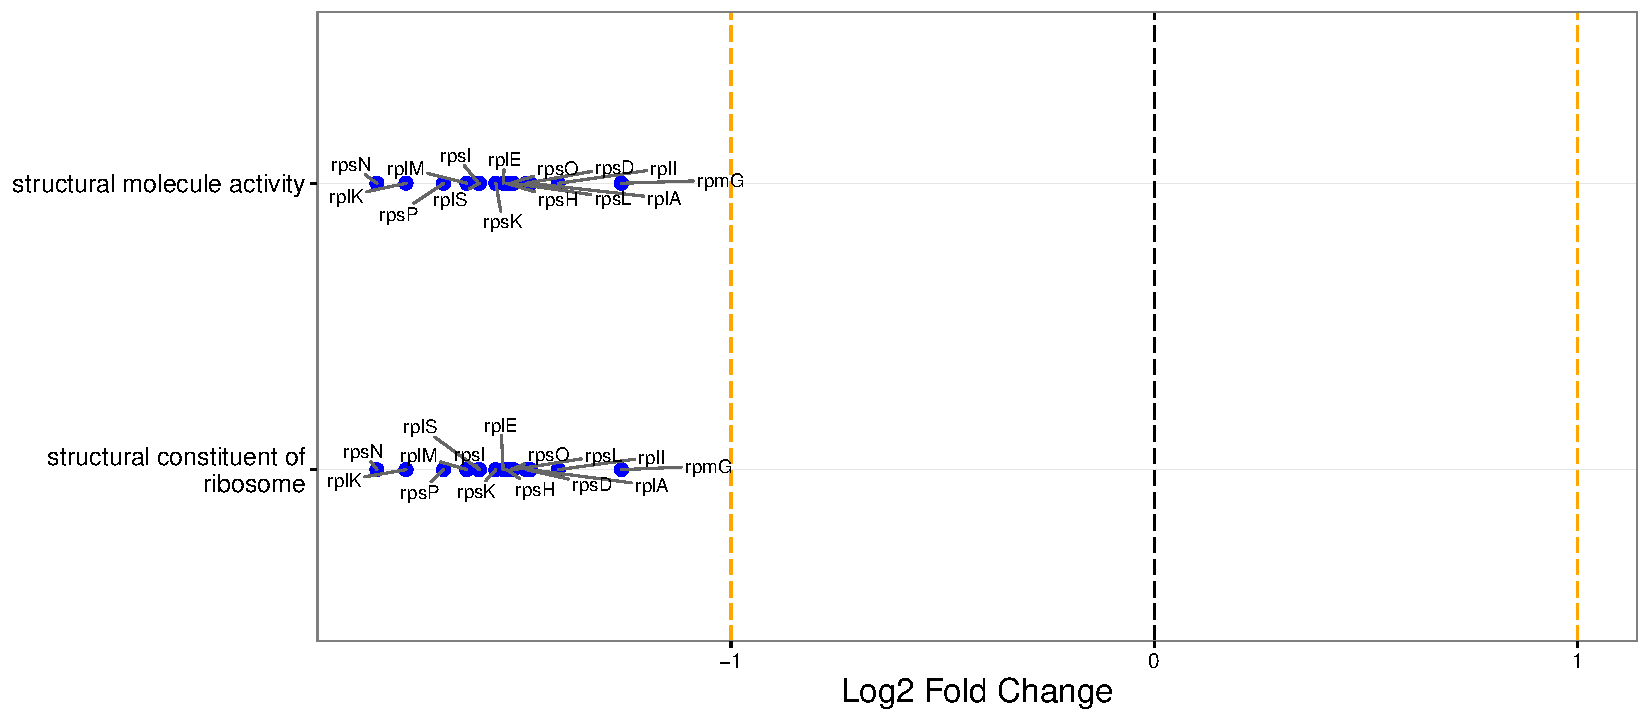
\includegraphics[width=1.0\textwidth]{../../d_figures/mf_n_03.pdf}
	\caption[Significantly altered GO annotations associated with molecular functions for mRNA samples in exponential phase tested for low Mg\textsuperscript{+2} against base Mg\textsuperscript{+2}]
	{\textbf{Significantly differentially expressed GO annotations related with molecular functions and associated genes with low Mg\textsuperscript{+2} levels in exponential phase, as determined by mRNA abundances.} The top differentially expressed KEGG pathways are shown along the y axis, and the relative fold change of the corresponding genes is shown along the x axis. We show up to 10 most significantly changed pathways and for each pathway, we show up to 15 of the most significantly changing genes.}
\end{figure}

\clearpage
\begin{figure}
	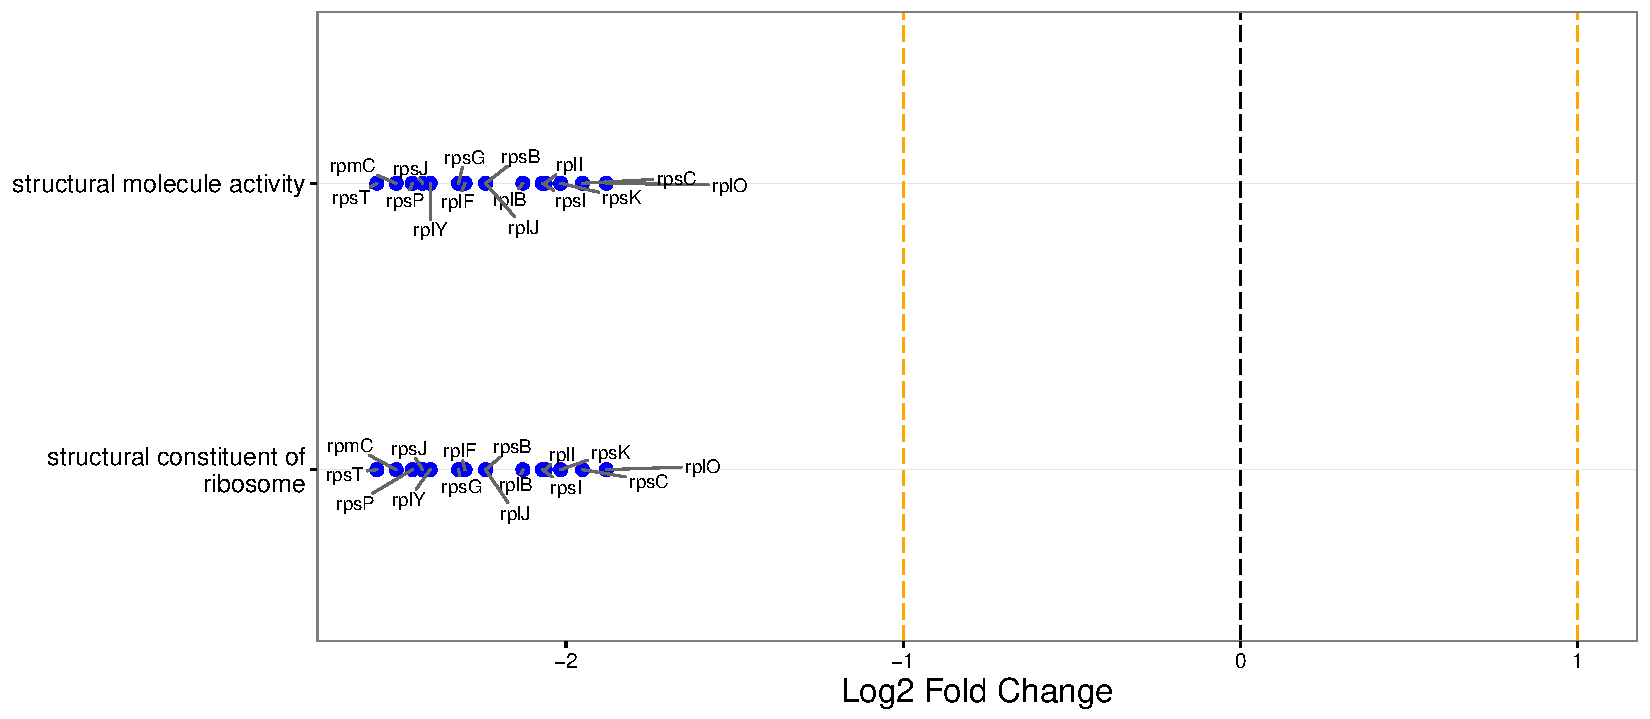
\includegraphics[width=1.0\textwidth]{../../d_figures/mf_n_04.pdf}
	\caption[Significantly altered GO annotations associated with molecular functions for protein samples in exponential phase tested for high Na\textsuperscript{+1} against base Na\textsuperscript{+1}]
	{\textbf{Significantly differentially expressed GO annotations related with molecular functions and associated genes with high Na\textsuperscript{+1} levels in exponential phase, as determined by protein abundances.} The top differentially expressed KEGG pathways are shown along the y axis, and the relative fold change of the corresponding genes is shown along the x axis. We show up to 10 most significantly changed pathways and for each pathway, we show up to 15 of the most significantly changing genes.}
\end{figure}

\clearpage
\begin{figure}
	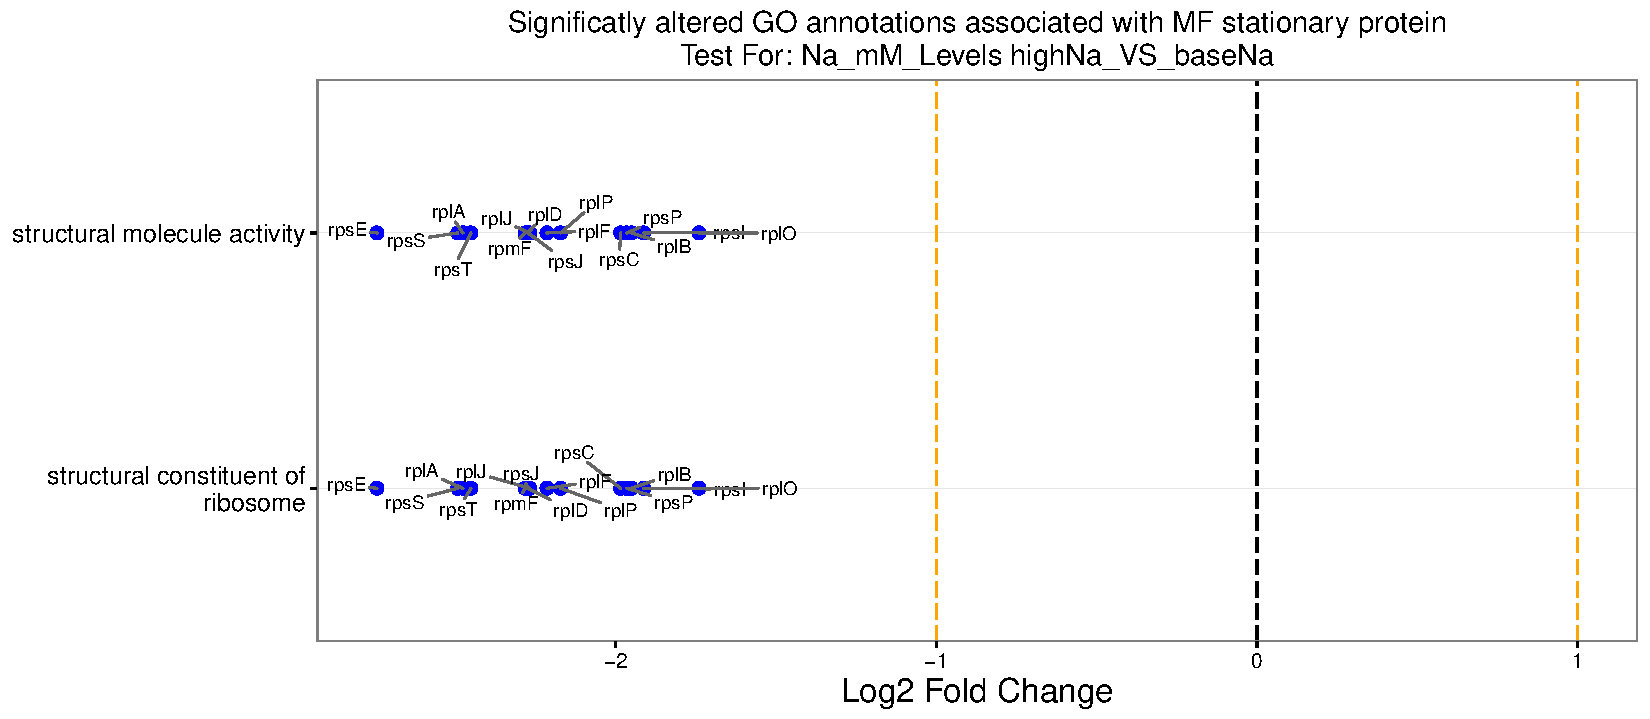
\includegraphics[width=1.0\textwidth]{../../d_figures/mf_n_05.pdf}
	\caption[Significantly altered GO annotations associated with molecular functions for protein samples in stationary phase tested for high Na\textsuperscript{+1} against base Na\textsuperscript{+1}]
	{\textbf{Significantly differentially expressed GO annotations related with molecular functions and associated genes with high Na\textsuperscript{+1} levels in stationary phase, as determined by protein abundances.} The top differentially expressed KEGG pathways are shown along the y axis, and the relative fold change of the corresponding genes is shown along the x axis. We show up to 10 most significantly changed pathways and for each pathway, we show up to 15 of the most significantly changing genes.}
\end{figure}

%\clearpage
%\begin{figure}[!htb]
%	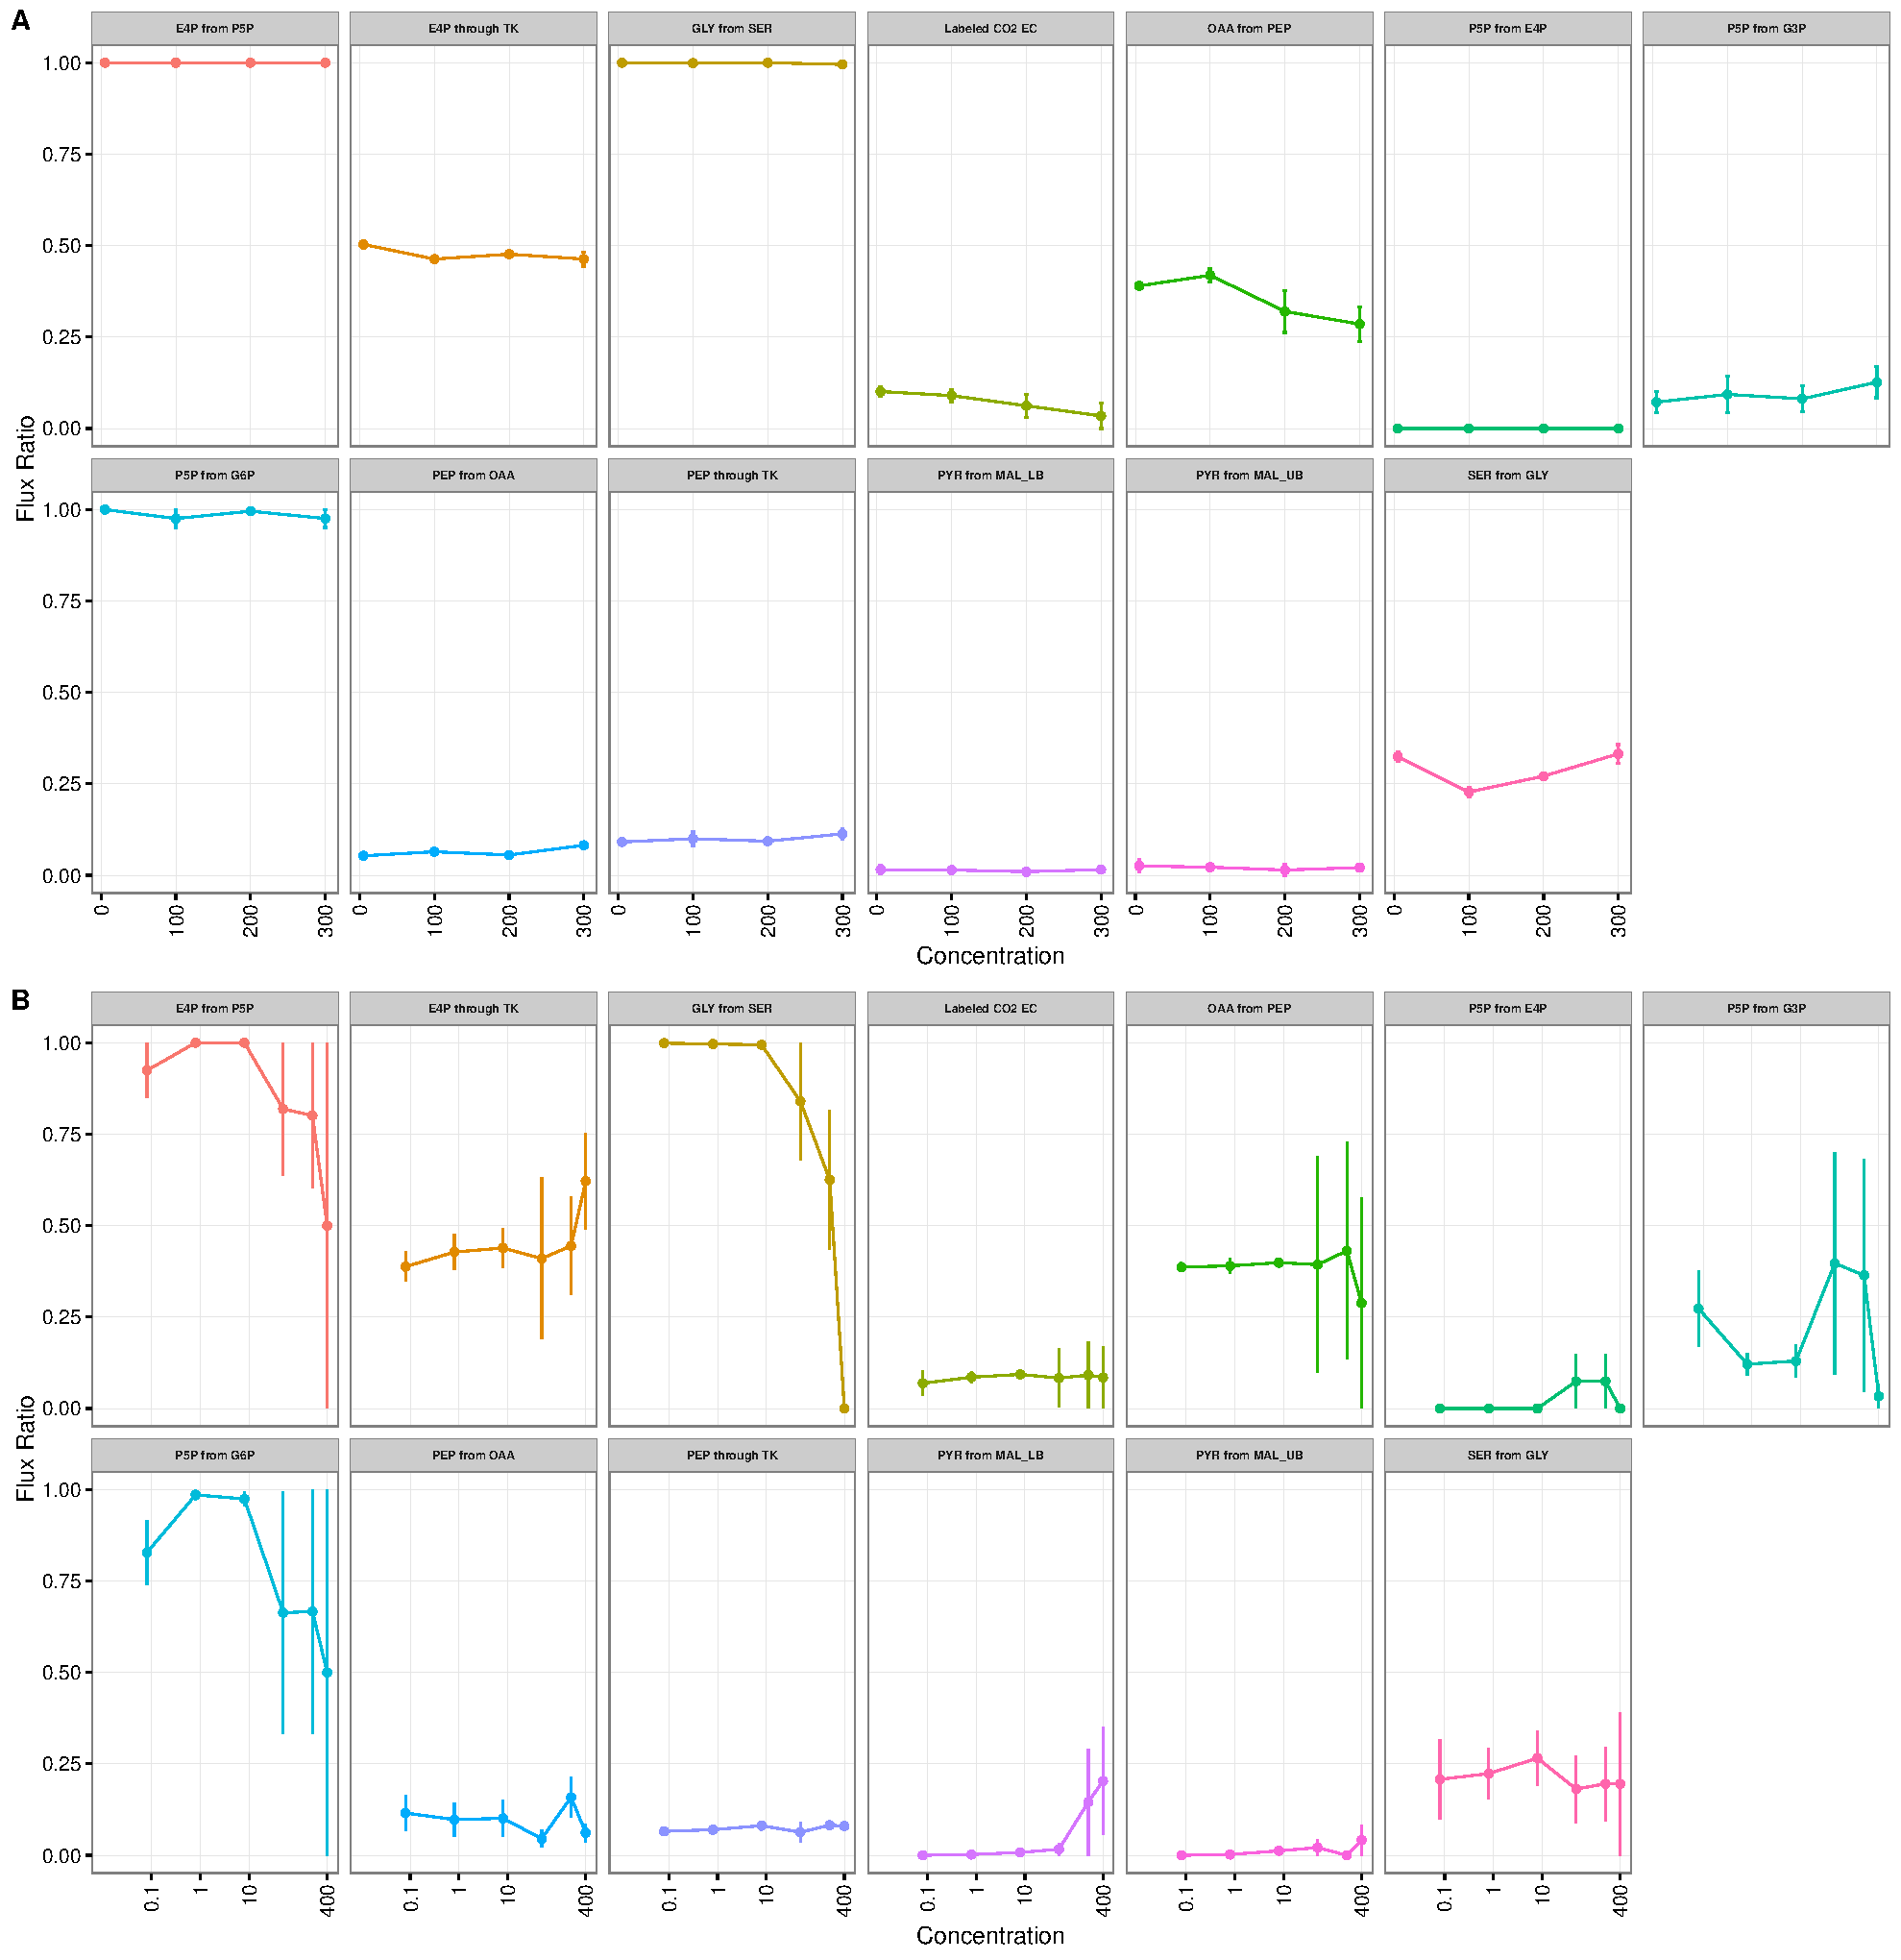
\includegraphics[width=1\textwidth]{../supplementary_figures/figS2_FluxSta.pdf}
%	\caption[Flux Stationary]
%	{\textbf{Flux changes with respect to salt stresses in stationary phase.} flux were measured with respect to four different Na and five different Mg concentrations. (A) Concentrations with respect to changing Na+ concentrations. (B) Concentrations with respect to changing Mg2+ concentrations.}
%\end{figure}


\end{document}